\documentclass[a4paper,12pt]{article}

% Самые необходимые пакеты
\usepackage[T2A]{fontenc}
\usepackage[utf8]{inputenc}
\usepackage[russian]{babel}
\usepackage{geometry}
\usepackage{amsmath}
\usepackage{graphicx}
\usepackage{float} 
\usepackage{xcolor}
\usepackage{listings}
\usepackage{hyperref}
\usepackage{array}
\usepackage{caption}
\usepackage{booktabs}
\usepackage{amssymb}
\usepackage{subcaption}
\usepackage{caption}
\captionsetup[figure]{name=Рисунок}
\captionsetup[table]{name=Таблица}
\usepackage{pgfplots}
\pgfplotsset{compat=1.18}
\usetikzlibrary{arrows.meta}
\usepackage{capt-of}
\usepackage{multirow}


\lstset{
	language=Matlab,
	basicstyle=\ttfamily\small,
	keywordstyle=\color{blue}\bfseries,
	commentstyle=\color{gray}\itshape,
	stringstyle=\color{red},
	numberstyle=\tiny\color{gray},
	numbers=left,
	stepnumber=1,
	numbersep=8pt,
	backgroundcolor=\color{white},
	frame=single,
	breaklines=true,
	breakatwhitespace=true,
	tabsize=4,
	showspaces=false,
	showstringspaces=false,
	captionpos=b,
	escapeinside={\%*}{*)}, % для вставки LaTeX кода внутри листинга
}
% Настройка геометрии
\geometry{left=1.5cm, right=2cm, bottom=2cm, top=2cm}

\begin{document}
	
	% Титульный лист
	\begin{titlepage}
		\centering
		\vspace*{1cm}
		
		% Министерство
		{\small
			Министерство науки и высшего образования Российской Федерации\\
			Федеральное государственное автономное образовательное учреждение\\
			высшего образования\\
			«Национальный исследовательский университет ИТМО»\\
		}
		
		\vspace{2cm}
		
		% Факультет
		{\large
			Факультет систем управления и робототехники\\
		}
		
		\vspace{3cm}
		
		% Основной заголовок
		{\Huge\bfseries
			ОТЧЕТ\\
		}
		\vspace{0.5cm}
		{\LARGE\bfseries
			о лабораторной работе №3\\
		}
		
		\vspace{1cm}
		
		% Дисциплина и тема
		{\Large
			По дисциплине: «Линейные системы автоматического управления»\\
			\vspace{0.5cm}
			Тема: «Вынужденное движение и показатели качества»\\
		}
		
		\vspace{3cm}
		
		% Информация о студенте и преподавателях
		\begin{minipage}{0.4\textwidth}
			\raggedright
			{\large
				Студент:\\
			}
			Охрименко Е. Д.\\
			Поток: 1.1.3\\
			Вариант: 17\\
		\end{minipage}
		\hfill
		\begin{minipage}{0.4\textwidth}
			\raggedleft
			{\large
				Преподаватель:\\
			}
			Пашенко А. В.\\
		\end{minipage}
		
		\vfill
		
		% Город и год
		{\large
			Санкт-Петербург\\
			2025\\
		}
		
	\end{titlepage}
	
	\newpage
	\tableofcontents
	
	\newpage
	\section{Задание. Вынужденное движение}
	
	Рассмотрю линейную систему второго порядка, заданную дифференциальным уравнением:
	
	\[
	\ddot{y} + a_1 \dot{y} + a_0 y = a_0 u(t)
	\]
	
	Требуется:
	
	\begin{itemize}
		\item Построить структурную схему системы с использованием элементарных блоков и отметить на ней узлы задания начальных условий \( y(0) \) и \( \dot{y}(0) \).
		\item Выполнить моделирование системы для нескольких наборов коэффициентов \( a_1 \) и \( a_0 \) при различных начальных условиях.
		\item Построить графики выходных сигналов \( y(t) \) для каждого варианта на одной координатной плоскости для наглядного сравнения.
		\item Сделать соответствующие выводы по результатам моделирования.
	\end{itemize}
	
	\subsection{Аналитические выкладки}
	
	В работе используются параметры коэффициентов \(a_1\) и \(a_0\), вычисленные в Лабораторной работе №2 (задания 2, 3, 4). Для удобства их значения сведены в таблицу \ref{tab:params}.
	
	\begin{table}[H]
		\centering
		\caption{Параметры экспериментов для варианта 17}
		\label{tab:params}
		\renewcommand{\arraystretch}{1.3}
		\begin{tabular}{@{}clccc@{}}
			\toprule
			\textbf{№ эксперимента} & \textbf{\(a_1\)} & \textbf{\(a_0\)} & \textbf{Начальные условия \(y(0), \dot{y}(0)\)} & \textbf{Вход \(u(t)\)} \\
			\midrule
			1 & 5.8 & 57.41 & \(-1, 0\);\quad \(0, 0\);\quad \(1, 0\) & \(0.5\) \quad \(0.8 t\) \quad \(\cos(2t)\)\\
			2 & 0 & 361 & \(-1, 0\);\quad \(0, 0\);\quad \(1, 0\) &\(0.5\) \quad \(0.8 t\) \quad \(\cos(2t)\) \\
			3 & -1.8 & 49.81 & \(-1, 0\);\quad \(0, 0\);\quad \(1, 0\) & \(0.5\) \quad \(0.8 t\) \quad \(\cos(2t)\) \\
			\bottomrule
		\end{tabular}
	\end{table}
	
	На графиках для каждого эксперимента будут представлены три траектории выхода \( y(t) \), соответствующие разным начальным условиям \( y(0) = -1, 0, 1 \) при фиксированном значении \(\dot{y}(0) = 0\). 
	
	
	
	\subsection{Структурная схема системы}
	
	Построю структурную схему системы -- возьму за основу схему из Лабораторной работы №2 (задание 1) и дострою вход \(u(t)\) с помощью блока \texttt{From Workspace}.
	
	\begin{figure}[H]
		\centering
		
\includegraphics[width=0.8\textwidth]{../images/task1/model1.png}
		\caption{Структурная схема системы}
	\end{figure}
	
	\subsection{Графики выходов}
	
	На графикaх экспериментов покажу выходные сигналы $y(t)$ при различных начальных условиях:
	\[
	y(0) = -1,\quad y(0) = 0,\quad y(0) = 1, \quad \dot{y}(0) = 0
	\]
	
	И при различных входных сигналах:
		
		\[u_1(t) = 0.5 \quad u_2(t) = 0.8t \quad u_3(t) = \text{cos}(2t) \]
		
	\subsubsection{Эксперимент 1}
	
	Для моделирования использованы параметры: \(a_1 = 5.8, \quad a_0 = 57.41\).
	
	\begin{figure}[H]
		\centering
		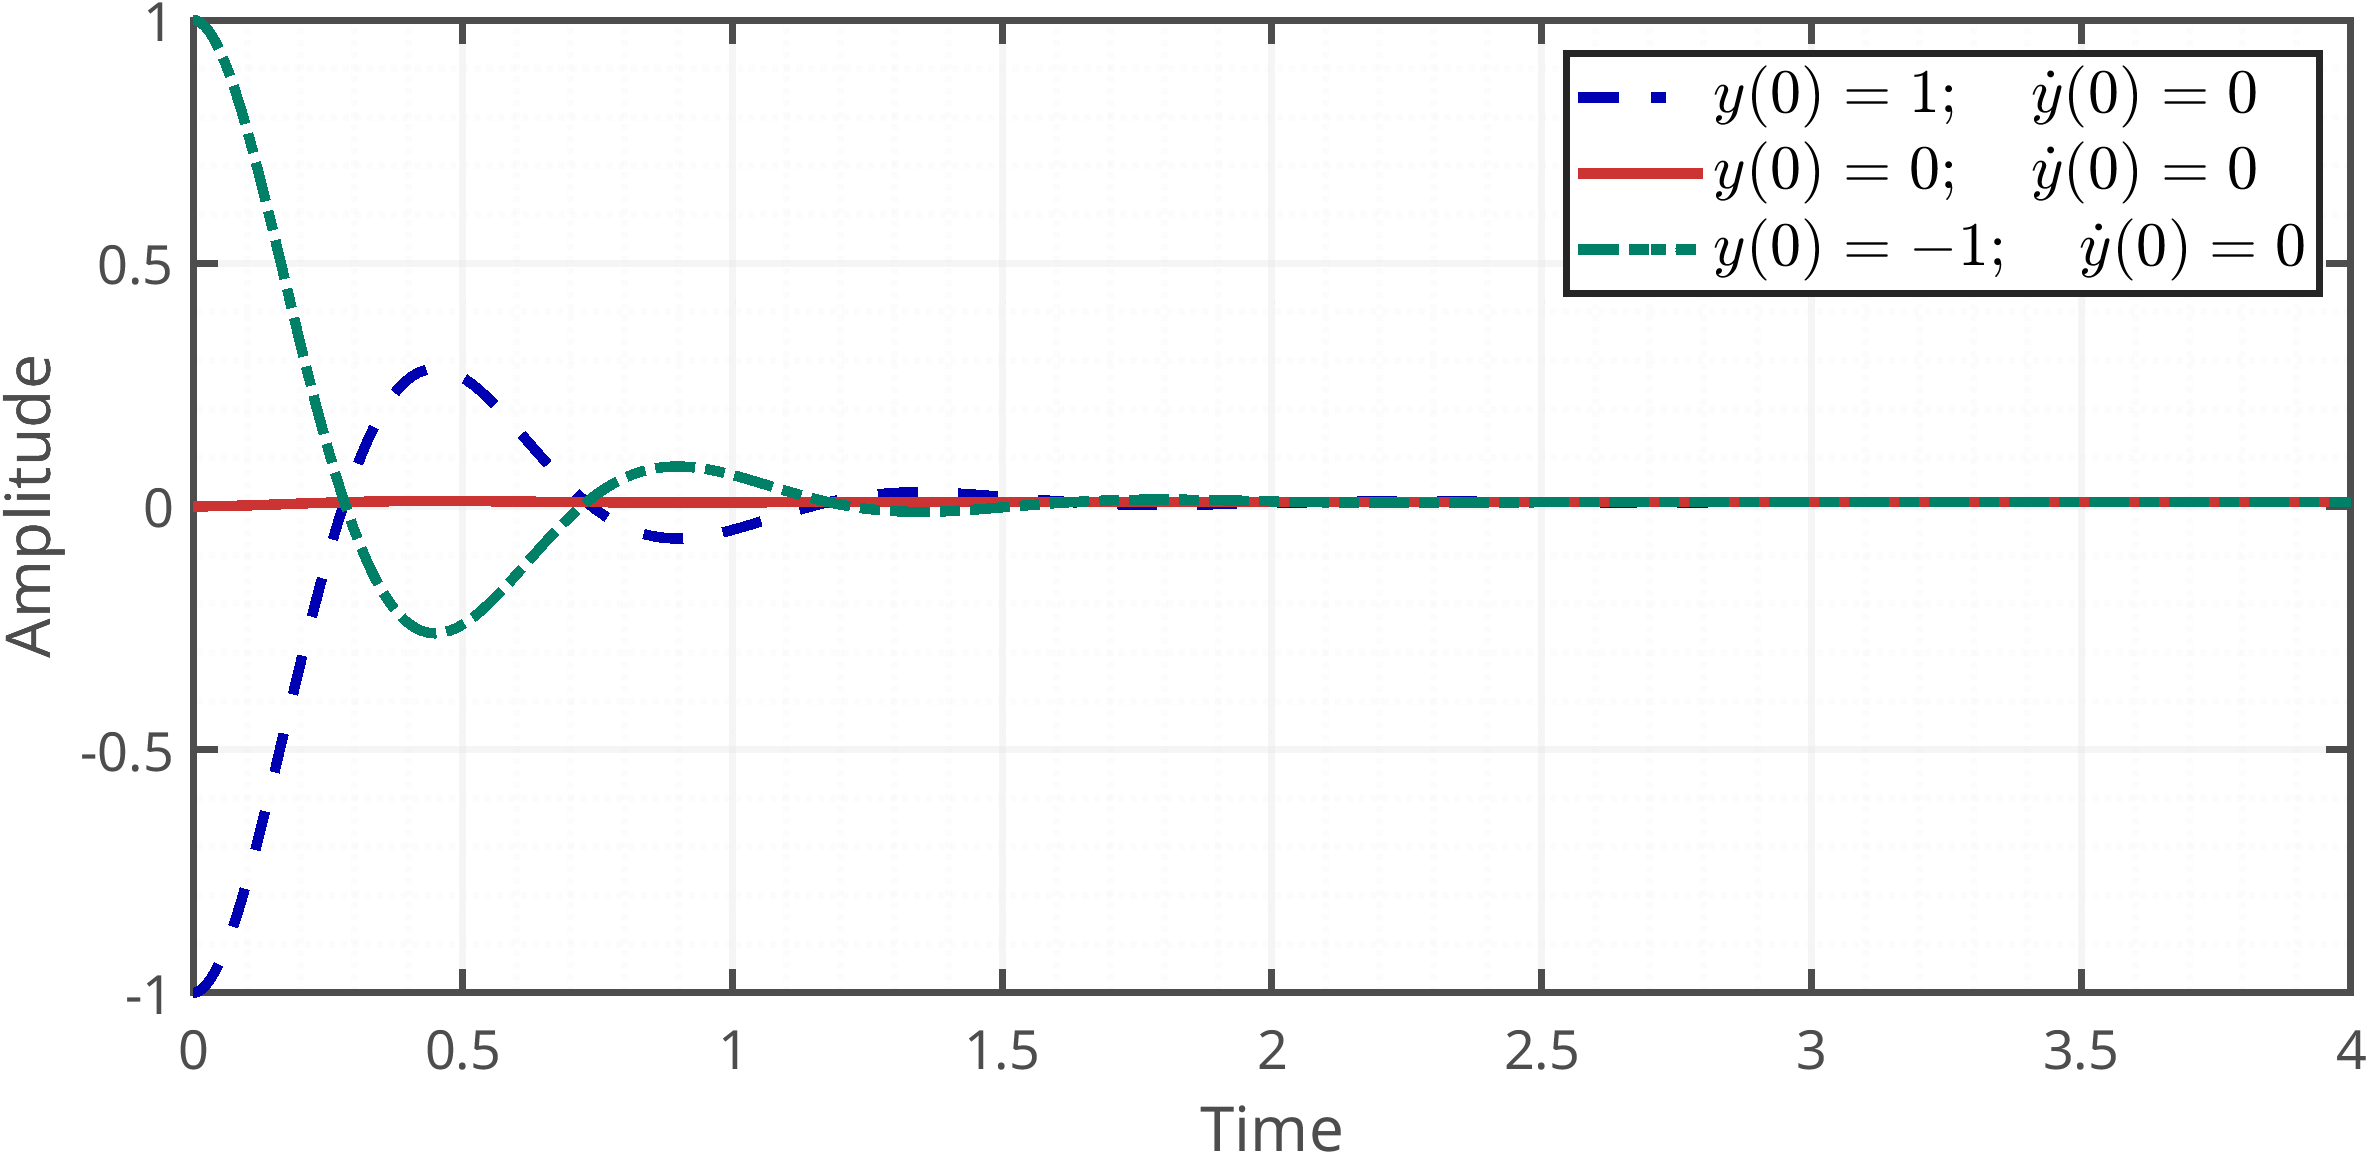
\includegraphics[width=0.9\textwidth]{../images/task1/y11.png}
		\caption{График сигналов при \(u_1(t) = 0.5\)}
	\end{figure}
	
	\begin{figure}[H]
		\centering
		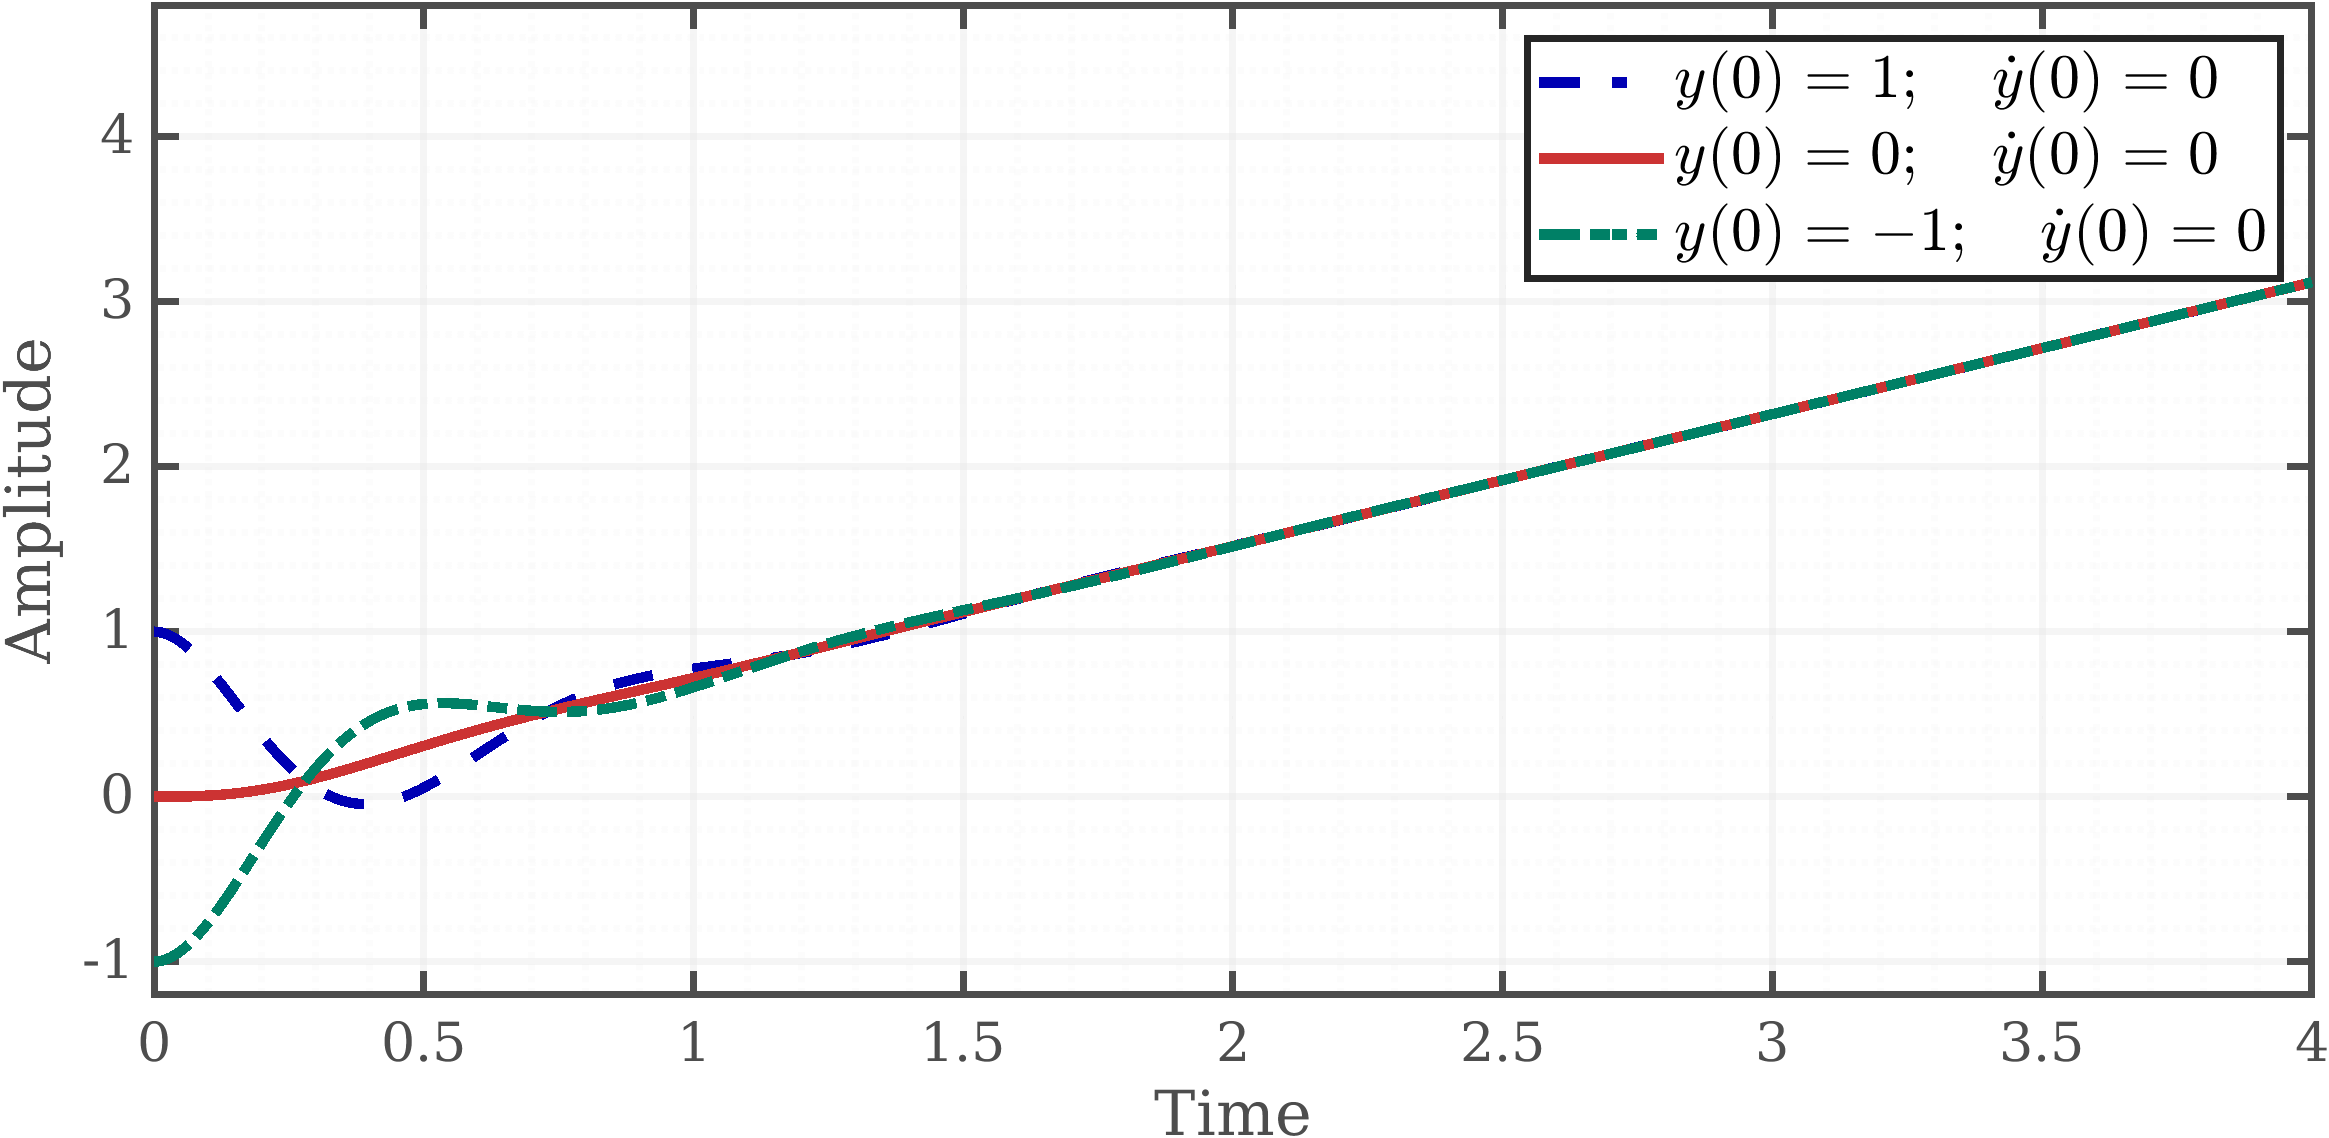
\includegraphics[width=0.9\textwidth]{../images/task1/y12.png}
		\caption{График сигналов при \(u_2(t) = 0.8 t\)}
	\end{figure}
	
	\begin{figure}[H]
		\centering
		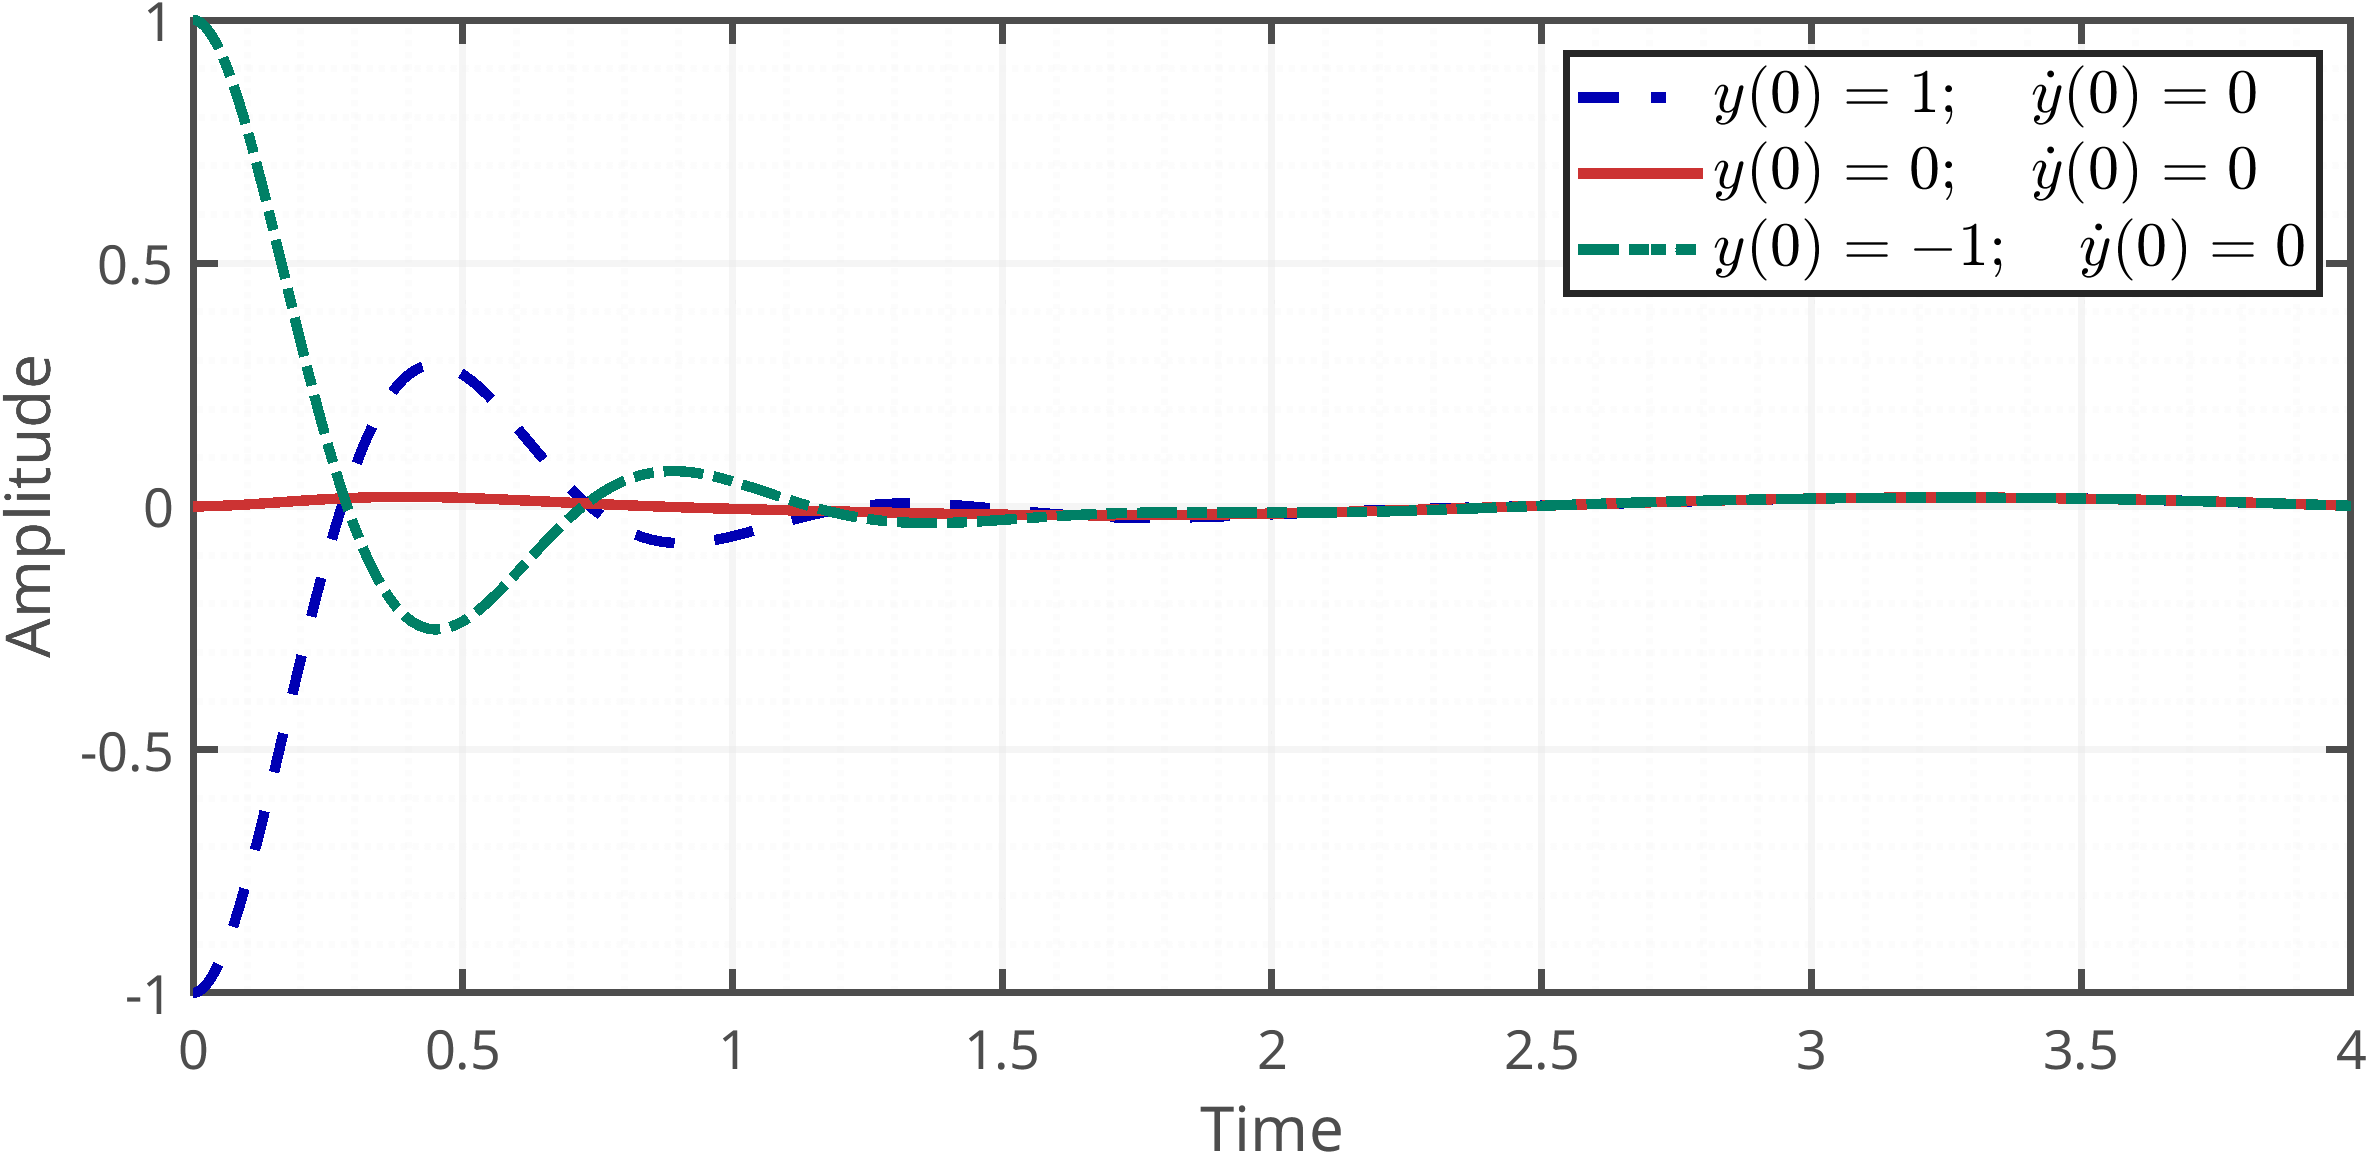
\includegraphics[width=0.9\textwidth]{../images/task1/y13.png}
		\caption{График сигналов при \(u_3(t) = \text{cos}(2t)\)}
	\end{figure}
	
	
	\subsubsection{Эксперимент 2}
	
	Для моделирования использованы параметры: \(a_1 = 0, \quad a_0 = 361\).
	
	\begin{figure}[H]
		\centering
		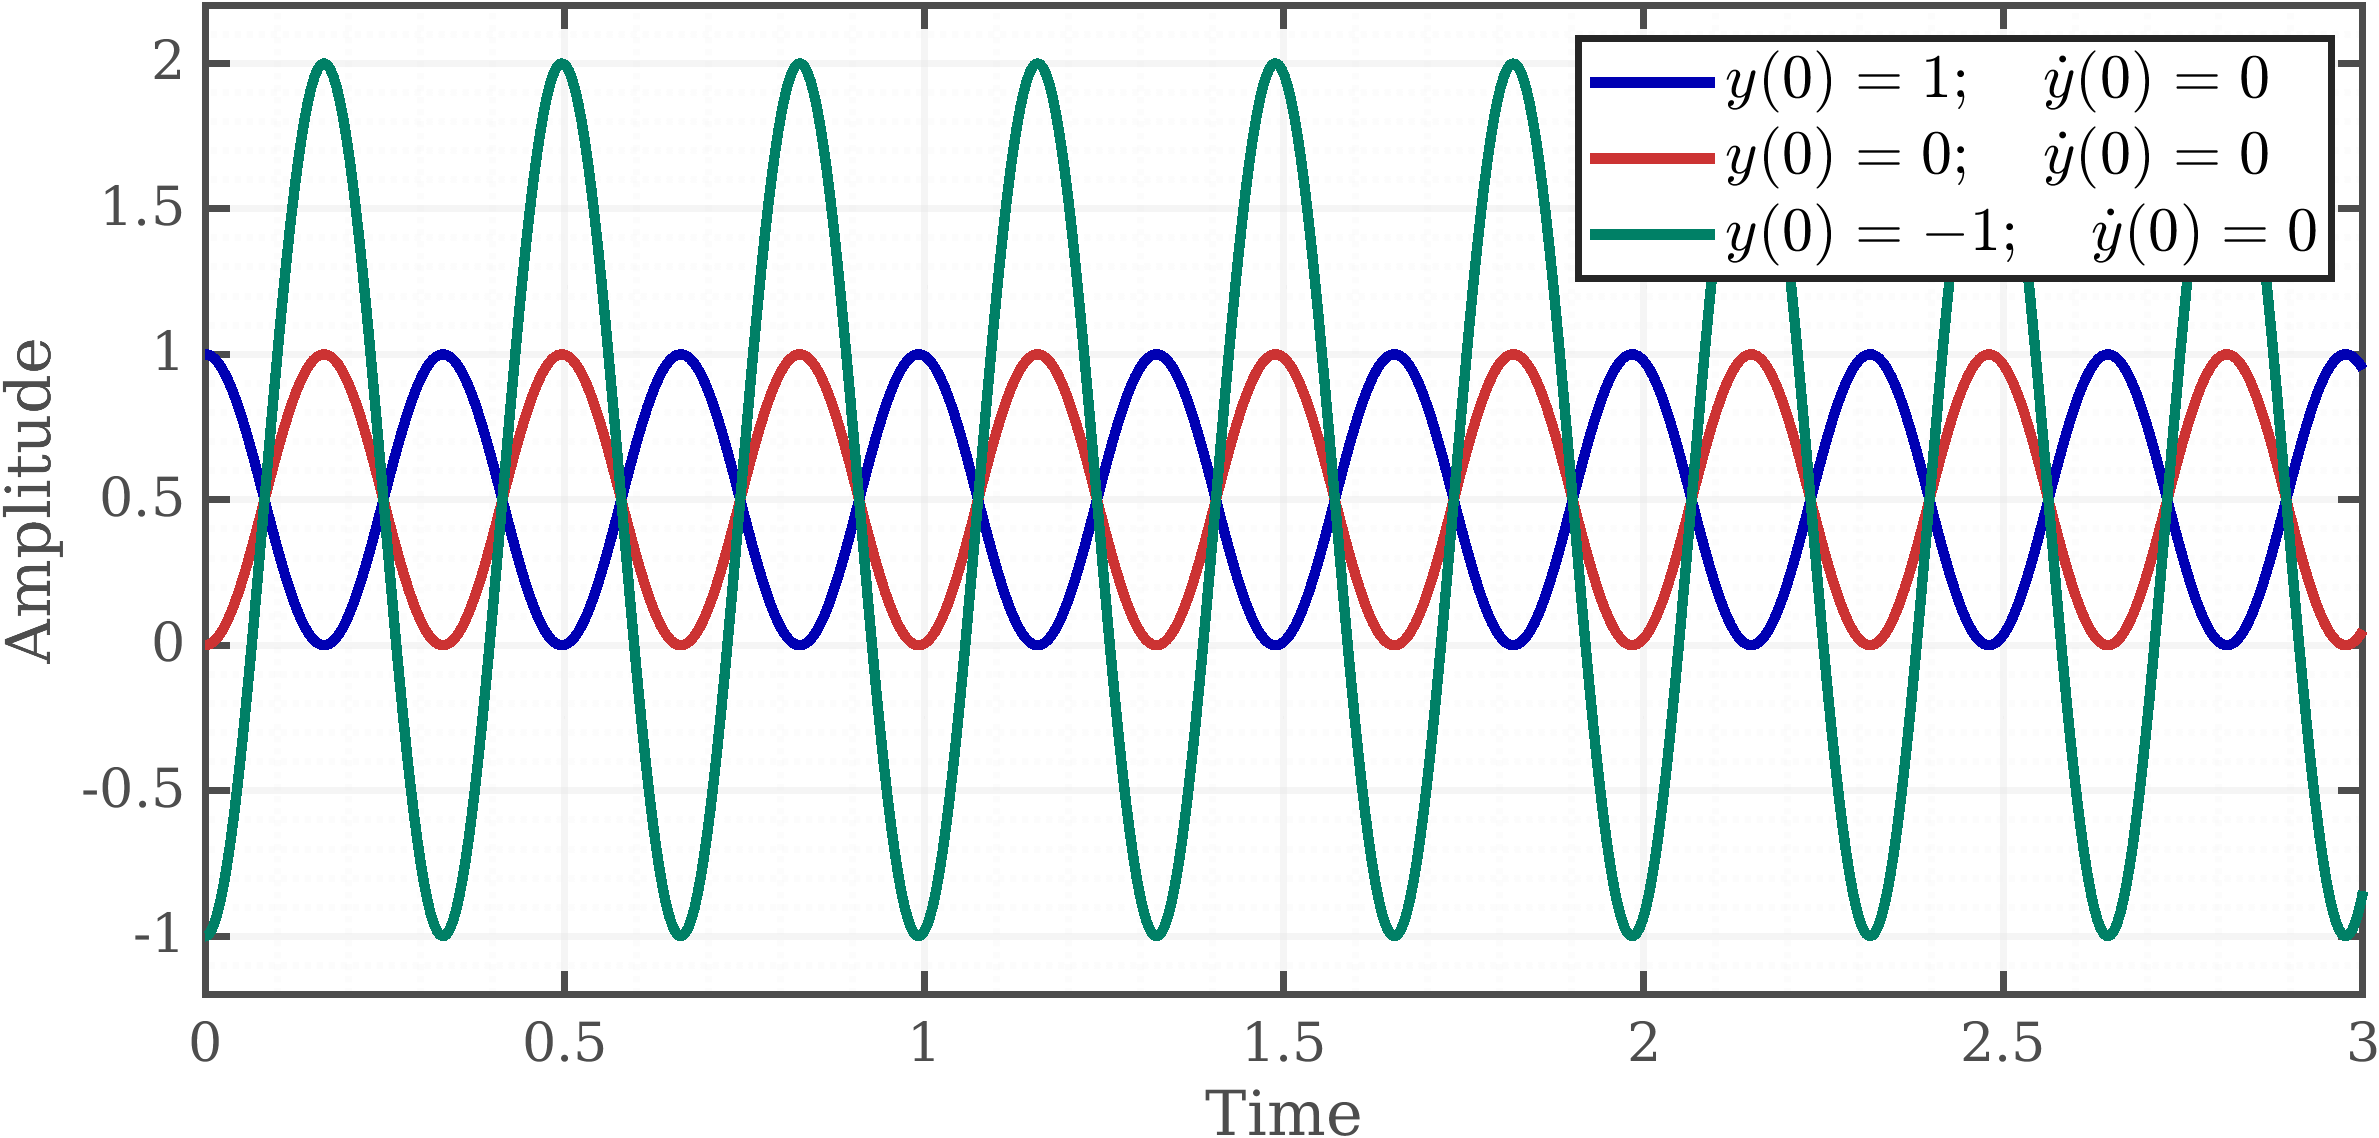
\includegraphics[width=0.9\textwidth]{../images/task1/y21.png}
		\caption{График сигналов при \(u(t) = 0.5\)}
	\end{figure}
	
	\begin{figure}[H]
		\centering
		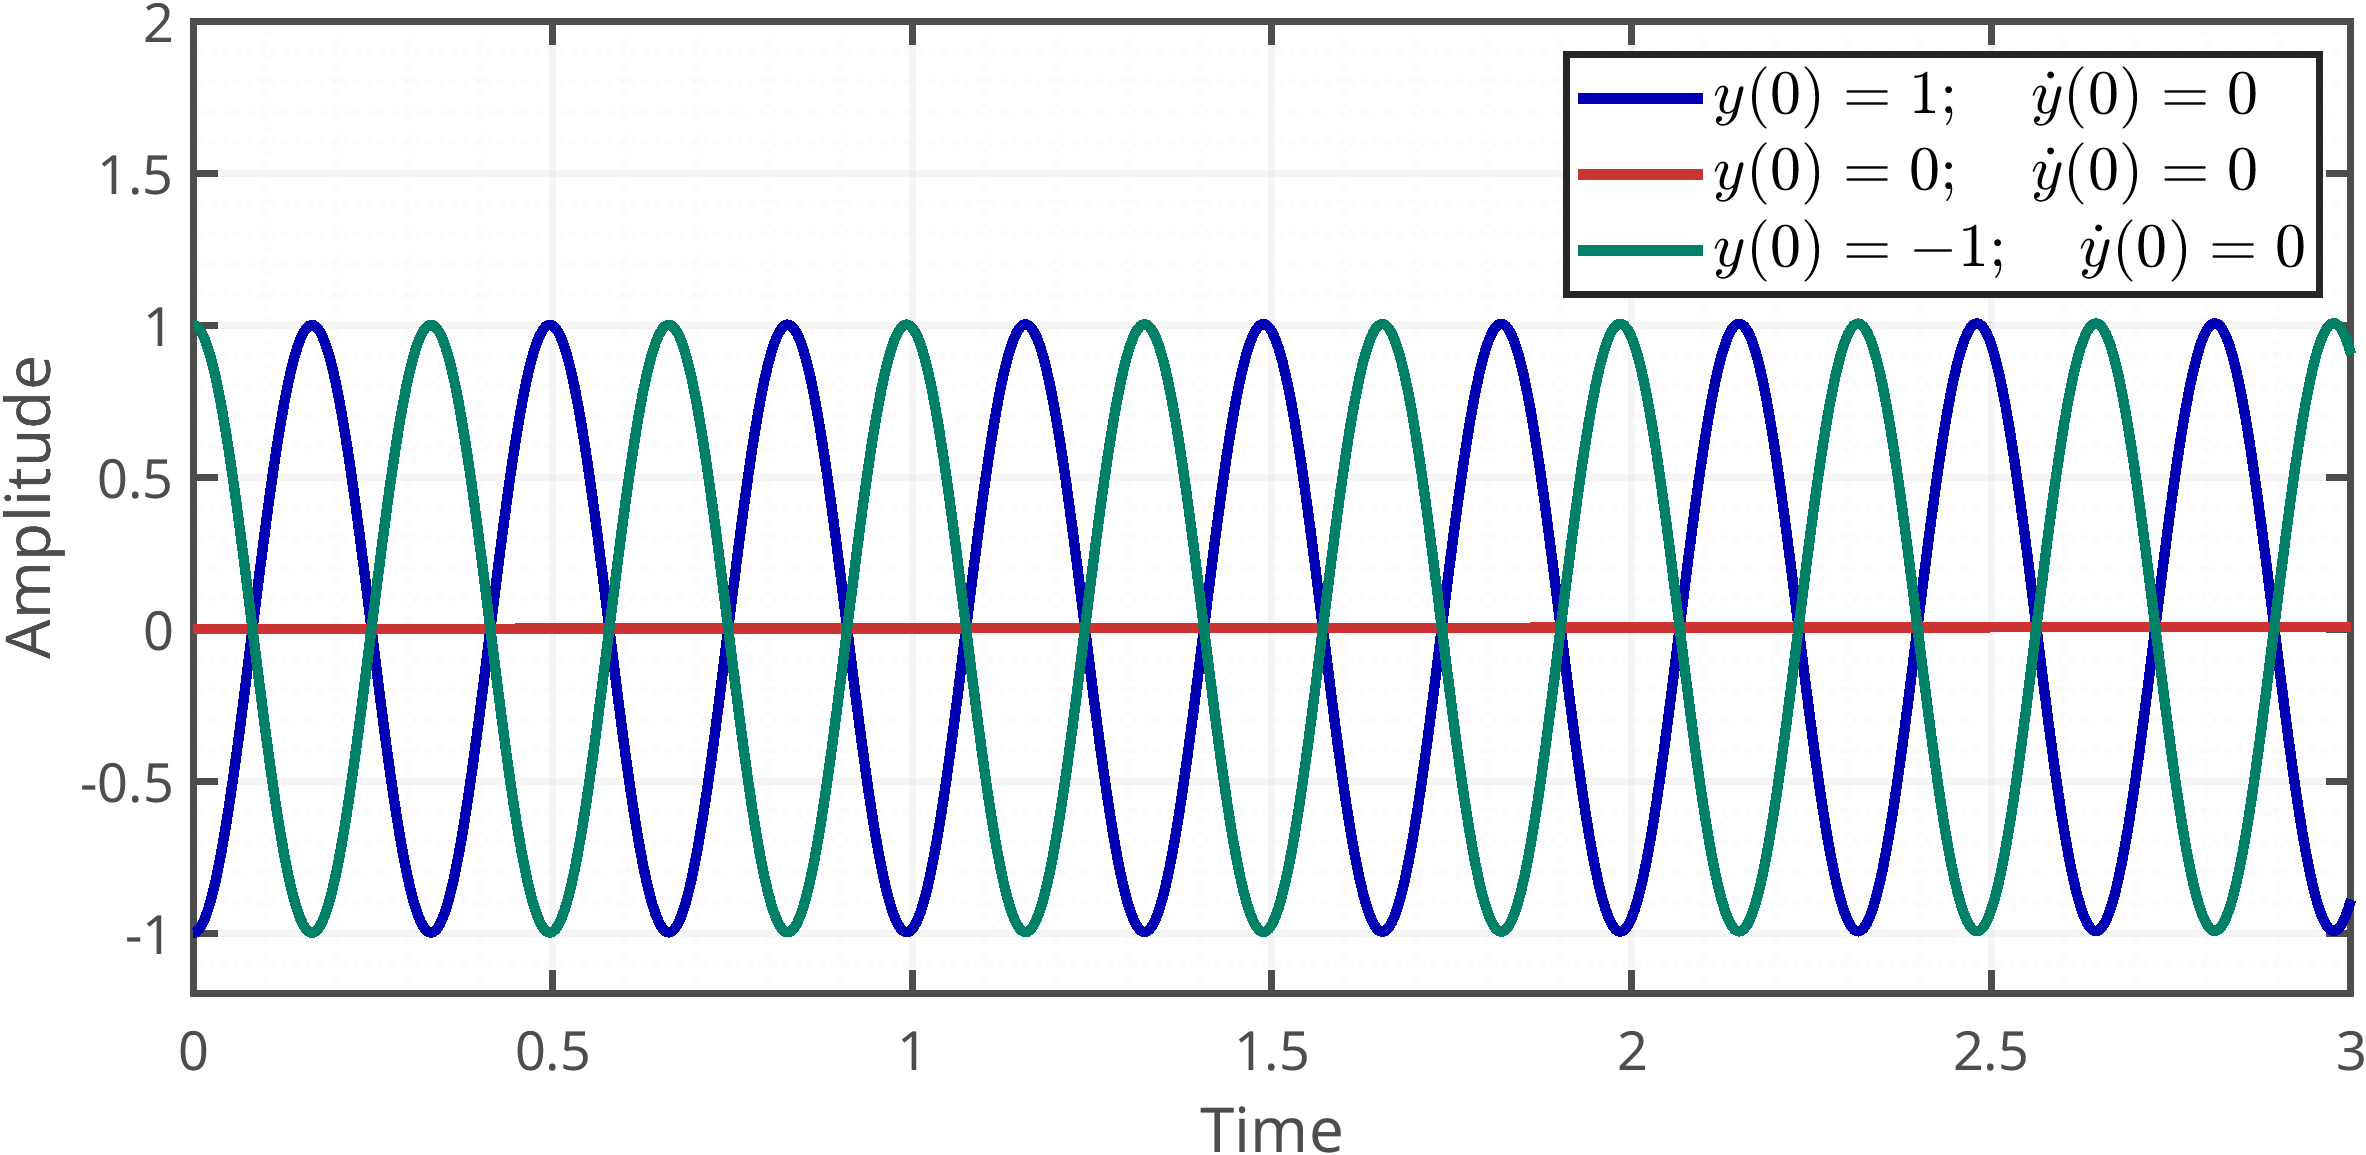
\includegraphics[width=0.9\textwidth]{../images/task1/y22.png}
		\caption{График сигналов при \(u(t) = 0.8 t\)}
	\end{figure}
	
	\begin{figure}[H]
		\centering
		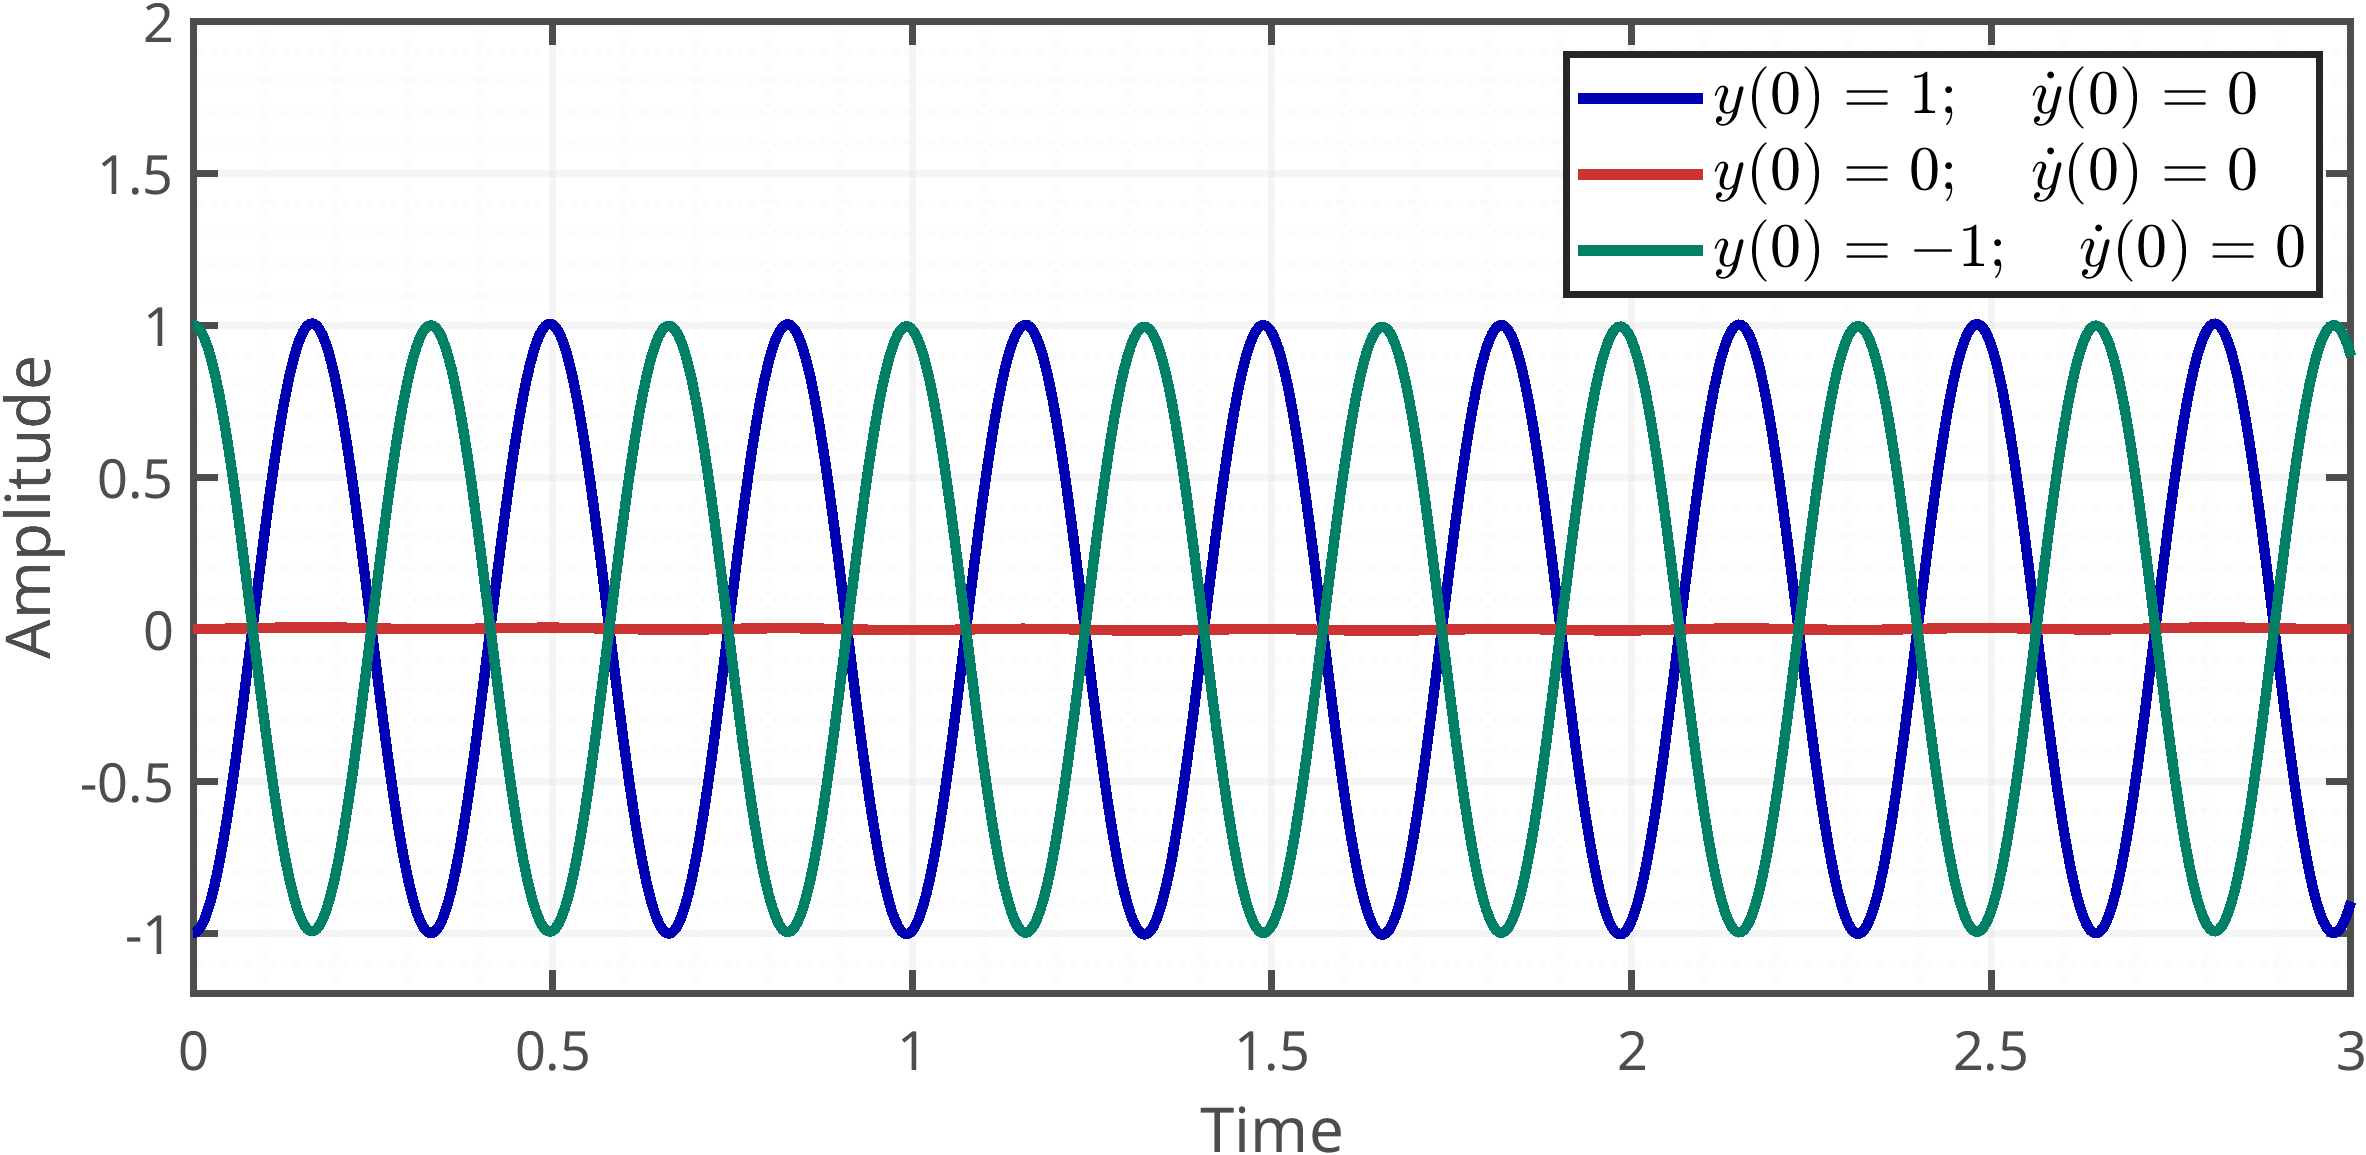
\includegraphics[width=0.9\textwidth]{../images/task1/y23.png}
		\caption{График сигналов при \(u(t) = \text{cos}(2t)\)}
	\end{figure}
	
	\subsubsection{Эксперимент 3}
	
	Для моделирования использованы параметры: \(a_1 = -1.8, \quad a_0 = 49.81\).
	
	\begin{figure}[H]
		\centering
		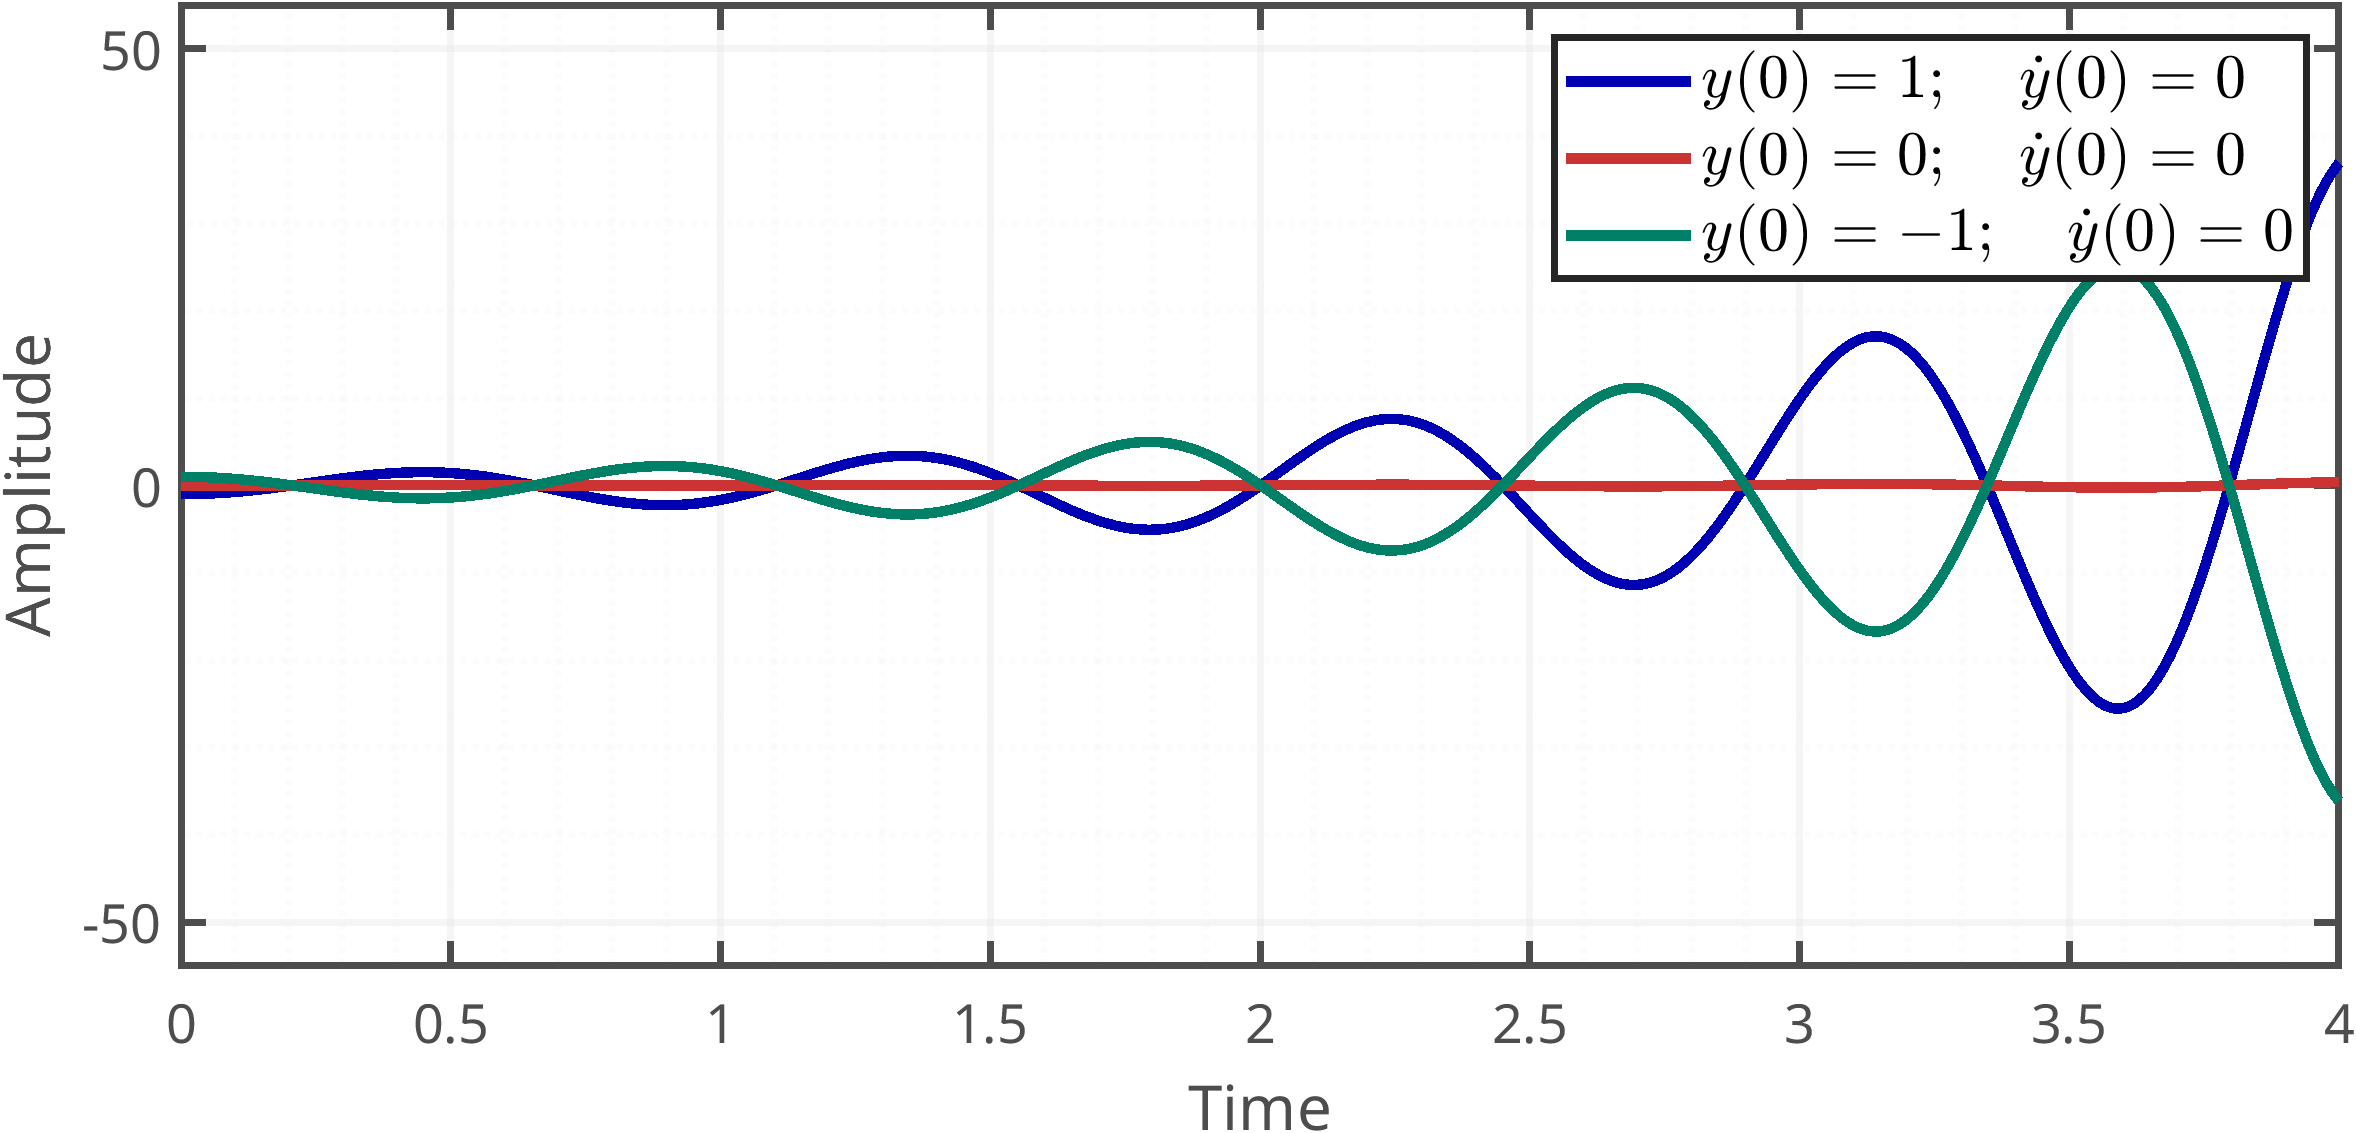
\includegraphics[width=0.9\textwidth]{../images/task1/y31.png}
		\caption{График сигналов при \(u(t) = 0.5\)}
	\end{figure}
	
	\begin{figure}[H]
		\centering
		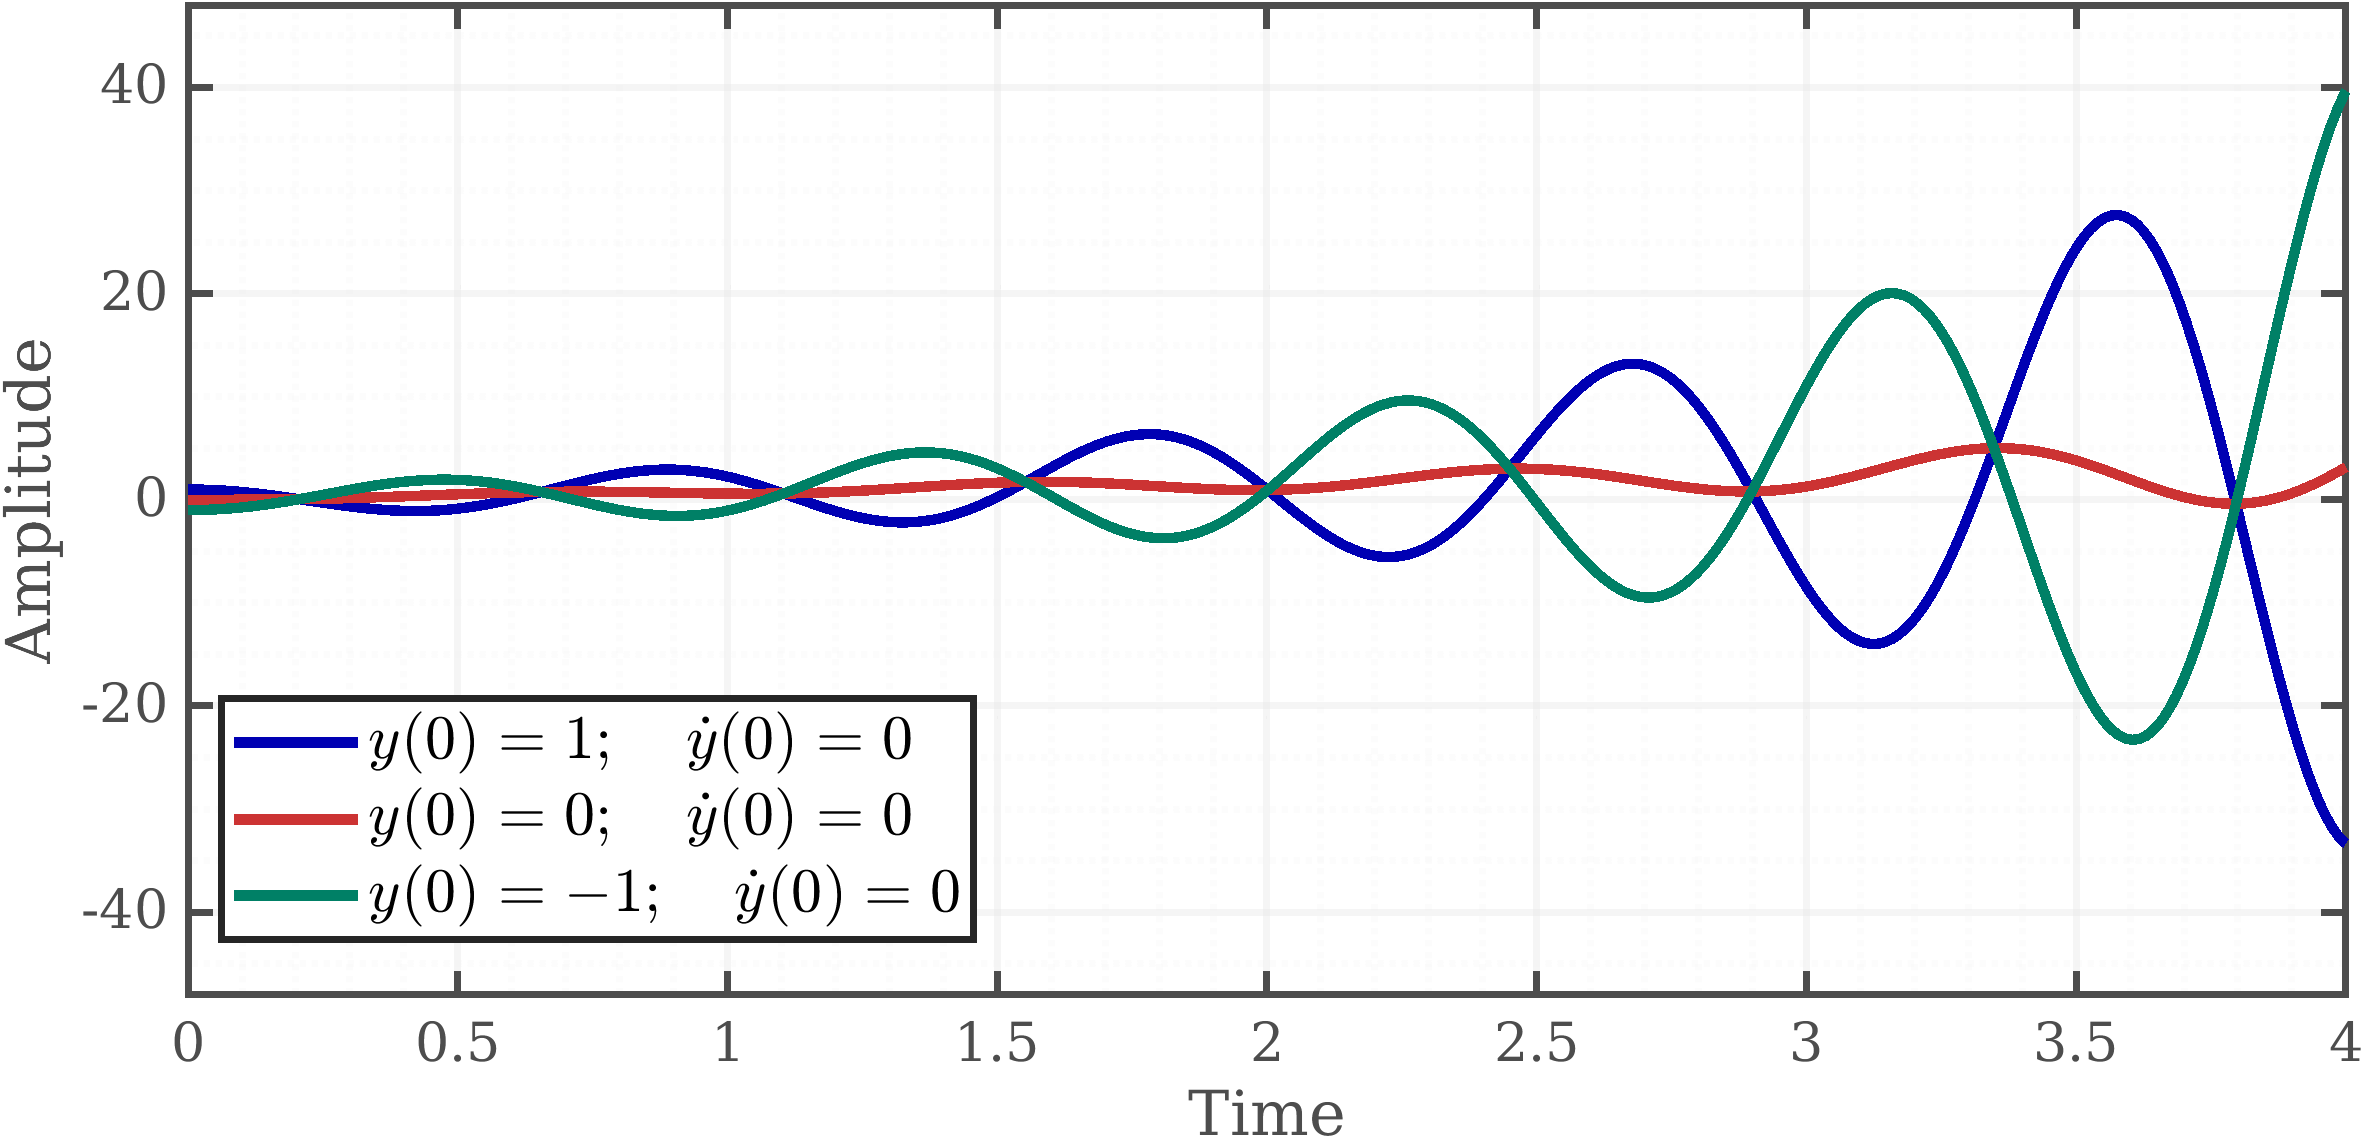
\includegraphics[width=0.9\textwidth]{../images/task1/y32.png}
		\caption{График сигналов при \(u(t) = 0.8 t\)}
	\end{figure}
	
	\begin{figure}[H]
		\centering
		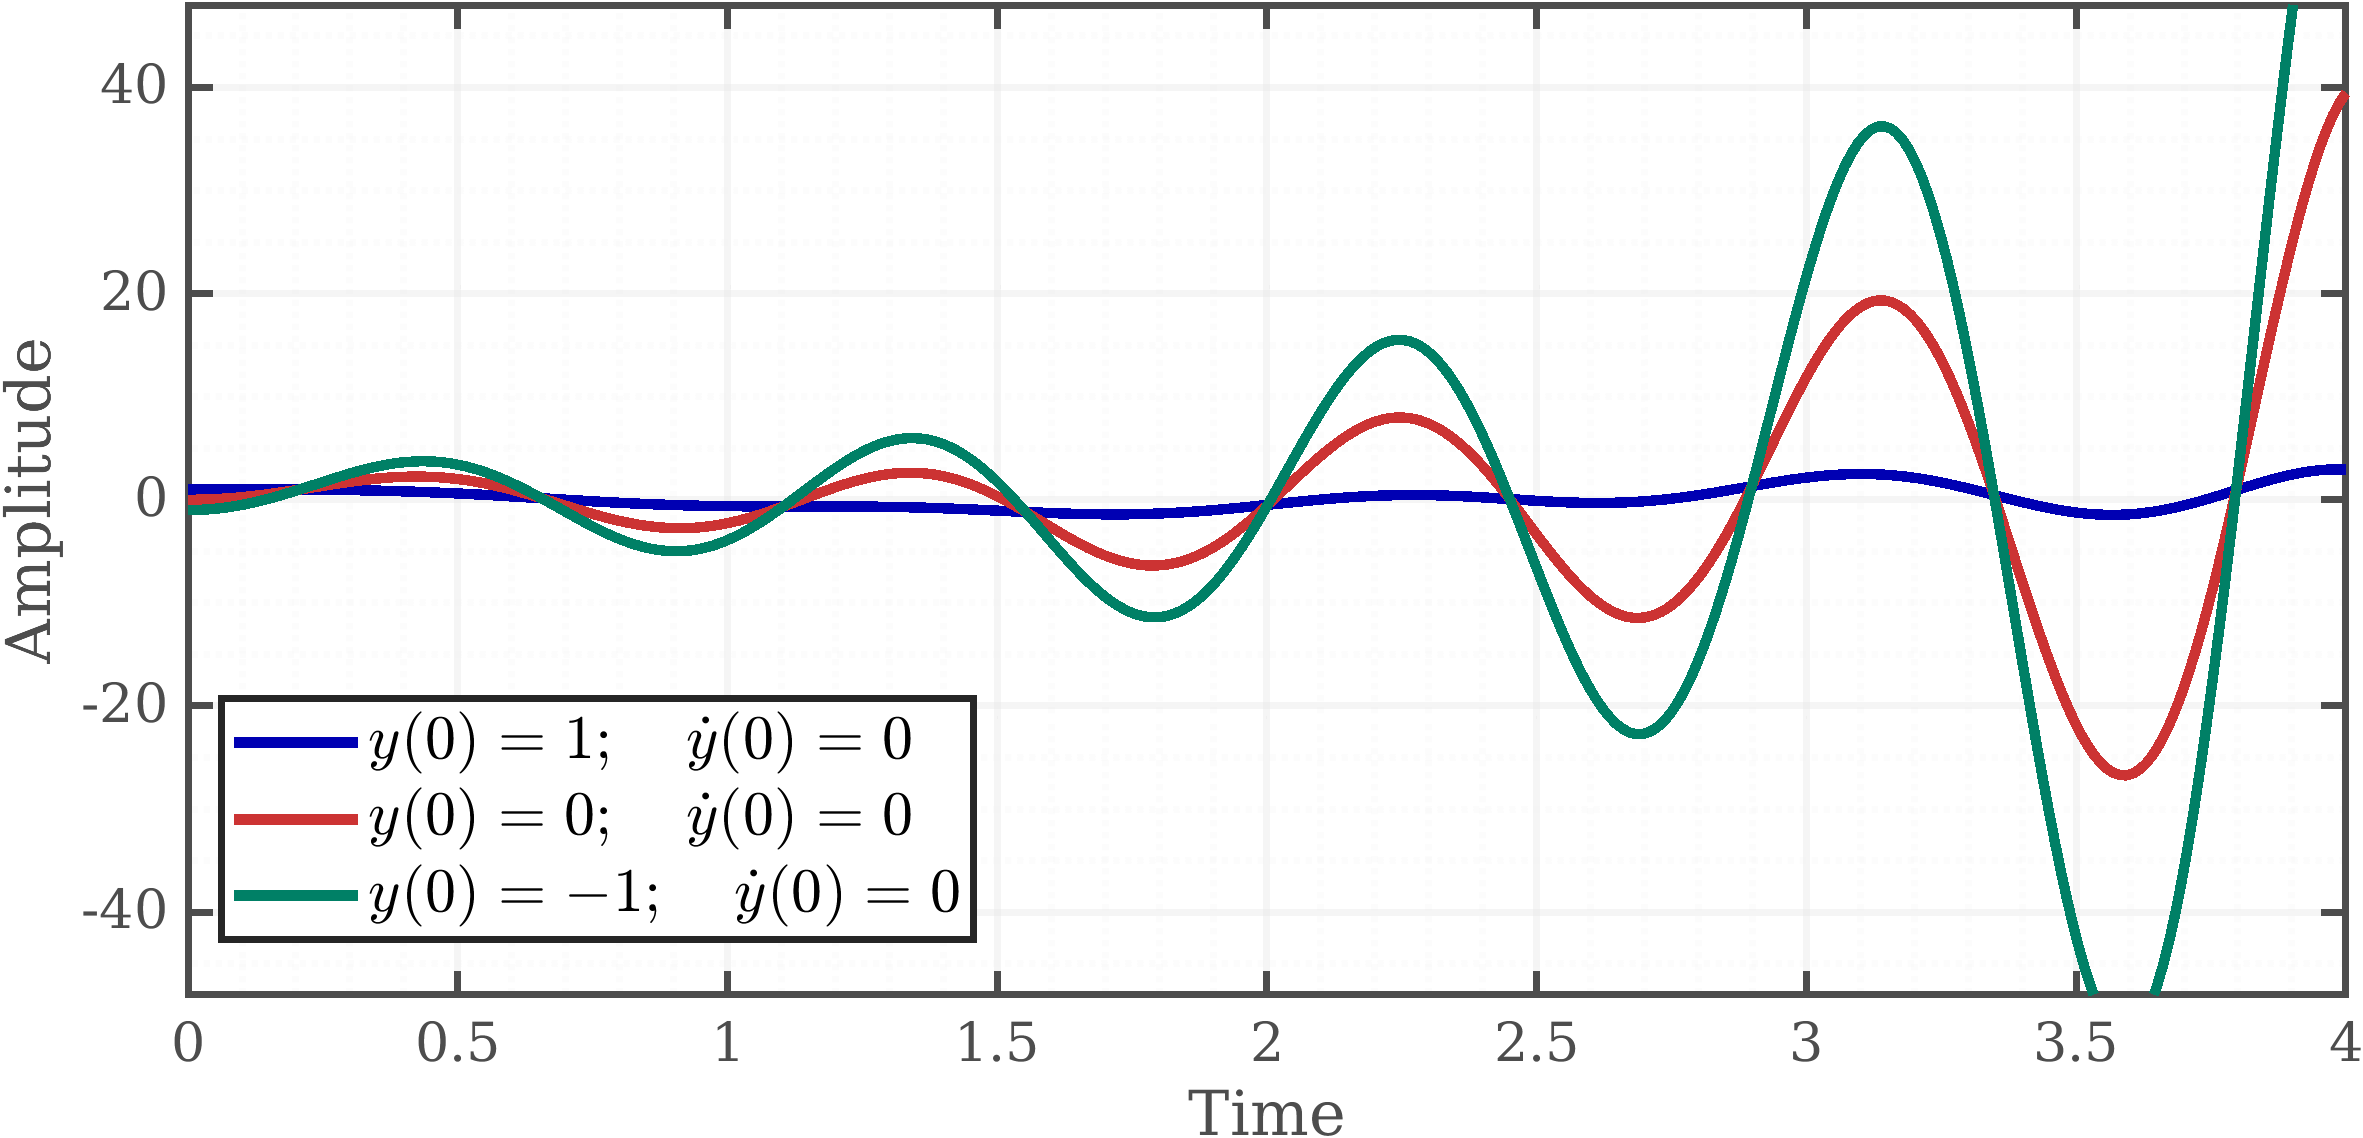
\includegraphics[width=0.9\textwidth]{../images/task1/y33.png}
		\caption{График сигналов при \(u(t) = \text{cos}(2t)\)}
	\end{figure}
	
	
	\textbf{Итог: }
	По графикам видно, что начальные условия задают исходное положение системы и влияют на её начальное поведение. При этом, в ходе проведённых экспериментов ни начальные условия, ни воздействующие сигналы не изменили устойчивость системы. Это подтверждает, что устойчивость определяется внутренними параметрами системы, а не внешними воздействиями или начальными условиями.
	
	
	
	

	\newpage
	\section{Задание. Качество переходных процессов}
	
	Рассмотрю линейную систему третьего порядка, заданную передаточной функцией:
	
	\[
	W(s) = \frac{|\lambda_1 \lambda_2 \lambda_3|}{(s - \lambda_1)(s - \lambda_2)(s - \lambda_3)},
	\]
	
	где \(\lambda_1, \lambda_2, \lambda_3\) — полюса с отрицательной вещественной частью.\\

	Требуется:
	
	\begin{itemize}
		\item Выбрать не менее шести наборов полюсов — половина вещественных, половина с комплексно-сопряжёнными.
		\item Смоделировать переходные процессы и построить графики переходных характеристик.
		\item Определить время переходного процесса и перерегулирование для каждого набора.
		\item Рассчитать степень колебательности и верхние оценки перерегулирования для комплексных полюсов.
		\item Сопоставить результаты и сделать выводы о влиянии полюсов на качество перехода.
		\item Визуализировать расположение корней на комплексной плоскости.
	\end{itemize}
	
	\subsection{Аналитические выкладки}
	
	Для исследования качества переходных процессов выберу восемь наборов полюсов, из которых четыре — с чисто вещественными корнями, и четыре — с комплексно-сопряжёнными. Для удобства помещу их в таблицу \ref{tab:poles_gost}.
	
	\begin{table}[H]
		\centering
		\caption{Наборы полюсов \(\lambda_1, \lambda_2, \lambda_3\) для системы 3-го порядка}
		\label{tab:poles_gost}
		\renewcommand{\arraystretch}{1.3}
		\begin{tabular}{c *{3}{>{\centering\arraybackslash}p{3cm}} >{\centering\arraybackslash}p{7cm}}
			\toprule
			\multicolumn{5}{c}{\textbf{Вещественные полюса}} \\
			\midrule
			№ & \(\lambda_1\) & \(\lambda_2\) & \(\lambda_3\) & \text{Примечание} \\
			\midrule
			1 & \(-1\)   & \(-1\)   & \(-1\)   & \(\lambda_1 = \lambda_2 = \lambda_3\) \\
			2 & \(-1\)   & \(-2\)   & \(-3\)   & \(\lambda_1 \neq \lambda_2 \neq \lambda_3\) \\
			3 & \(-0.5\) & \(-0.5\) & \(-10\)  & \(\lambda_3 \ll \lambda_1, \lambda_2\) \\
			4 & \(-0.1\) & \(-1\)   & \(-5\)   & разбросанные значения \\
			\midrule
			\multicolumn{5}{c}{\textbf{Комплексно-сопряжённые полюса (\(\lambda_{1,2} = \alpha \pm i \beta, \quad \alpha, \beta \in \mathbb{R} ,\quad \beta \neq 0)\)}} \\
			\midrule
			5 & \(-1 + 2i\)   & \(-1 - 2i\)   & \(-5\)    & \(\lambda_3 \in \mathbb{R}\) \\
			6 & \(-0.5 + 3i\) & \(-0.5 - 3i\) & \(-1\) & \(\lambda_3 \in \mathbb{R}\) \\
			7 & \(-0.1 + 1i\) & \(-0.1 - 1i\) & \(-0.5\)  & \(\alpha \approx 0\), близко к устойчивости \\
			8 & \(-1 + 1i\) & \(-1 - 1i\) & \(-0.05\) & \(\lambda_3 \approx 0\) \\
			\bottomrule
		\end{tabular}
	\end{table}
	
	
	Далее я проведу моделирование переходных процессов для каждого набора полюсов и оценю время переходного процесса и перерегулирование.
	\[\]
	Для системы с вещественными полюсами приведу в отчете:
	
	\begin{itemize}
		\item Перерегулирование $M_p$ — максимальное превышение выхода над установившимся значением:
		\[
		M_p = \frac{y_{\max} - y_{\infty}}{y_{\infty}} \cdot 100\%,
		\]
		где $y_{\max}$ — максимум отклика, $y_{\infty}$ — установившееся значение.
		
		\item Время переходного процесса $t_p$ — время, после которого отклик остаётся в пределах $\pm5\%$ от $y_{\infty}$:
		\[
		y(t) \in [0.95\, y_{\infty},\, 1.05\, y_{\infty}], \quad t \geq t_p.
		\]
		
			Допуск в 5\% — стандартный критерий, который хорошо показывает, когда система практически достигла устойчивого состояния, не обращая внимания на мелкие колебания.
			
	\end{itemize}
	 А для системы с комплексно-сопряженными полюсами приведу в отчете также и:
	 
		\begin{itemize}
			
			\item Сравнение верхней оценки перерегулирования с полученными значениями перерегулирования.
			
			\item Верхняя оценка перерегулирования:
			\[
			M_p^{\max} = e^{-\frac{\pi |\alpha|}{\beta}} \times 100\%,
			\]
			
			где \(\alpha\) и \(\beta\) — вещественная и мнимая части комплексно-сопряжённых полюсов \(\lambda = \alpha \pm i \beta\).
			
			
		\end{itemize}

	
	\subsection{Графики}
	
	На графиках показан переходной процесс системы с заданными полюсами.
	
	Синяя линия — отклик системы $y(t)$.
	
	Синяя полоса — область допустимых колебаний выходного сигнала в пределах $\pm 5\%$ от установившегося значения $y_\infty$.
	
	Красная пунктирная линия показывает время переходного процесса $t_p$ — момент, начиная с которого выходной сигнал остаётся в пределах этой зоны.
	
	Чёрные пунктирные линии отображают установившееся значение $y_\infty$ и максимальное значение отклика $y_{\max}$ (если $y_{\max} > y_\infty$).

	
	
	\subsubsection{Эксперимент 1}
	
	
	\begin{figure}[H]
		\centering
		\begin{minipage}[c]{0.66\textwidth}
			\centering
			\raisebox{-0.5\height}{
\includegraphics[width=\textwidth]{../images/task2/y1.png}}
		\end{minipage}
		\hfill
		\begin{minipage}[c]{0.31\textwidth}
			\centering
			\raisebox{0.2\height}{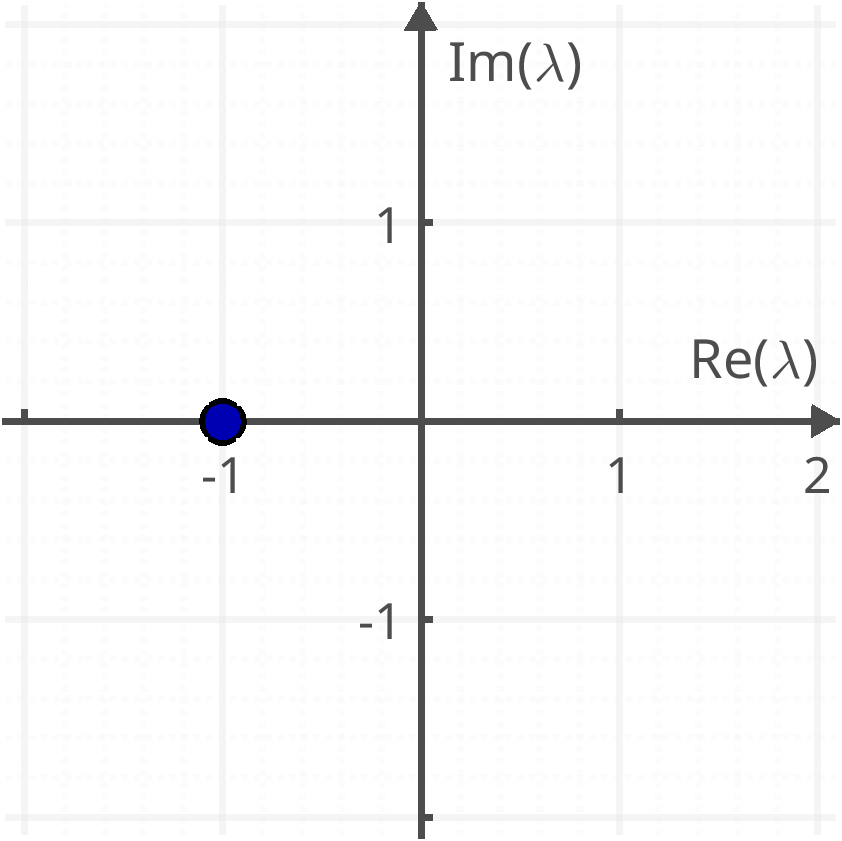
\includegraphics[width=\textwidth]{../images/task2/lambda1.png}}
		\end{minipage}
		
		\vspace{2mm} 
		
		\begin{minipage}[t]{0.68\textwidth}
			\centering
			\refstepcounter{figure}
			\small Рисунок~\thefigure: График выхода
		\end{minipage}
		\hfill
		\begin{minipage}[t]{0.29\textwidth}
			\centering
			\refstepcounter{figure}
			\small Рисунок~\thefigure: Полюса передаточной функции
		\end{minipage}
	\end{figure}
	
	
	Для эксперимента с полюсами
	\[
	\lambda = [-1, -1, -1]
	\]
	получены следующие характеристики переходного процесса:

	\[
	M_p = \frac{y_{\max} - y_{\infty}}{y_{\infty}} \times 100\% = \frac{1 - 1}{1} \times 100\% = 0\%
	\]
	
	
	\[
	t_p = 6.23 \text{ с}.
	\]
	
	
	
	\subsubsection{Эксперимент 2}
	
	
	\begin{figure}[H]
		\centering
		\begin{minipage}[c]{0.66\textwidth}
			\centering
			\raisebox{-0.5\height}{
\includegraphics[width=\textwidth]{../images/task2/y2.png}}
		\end{minipage}
		\hfill
		\begin{minipage}[c]{0.31\textwidth}
			\centering
			\raisebox{0.2\height}{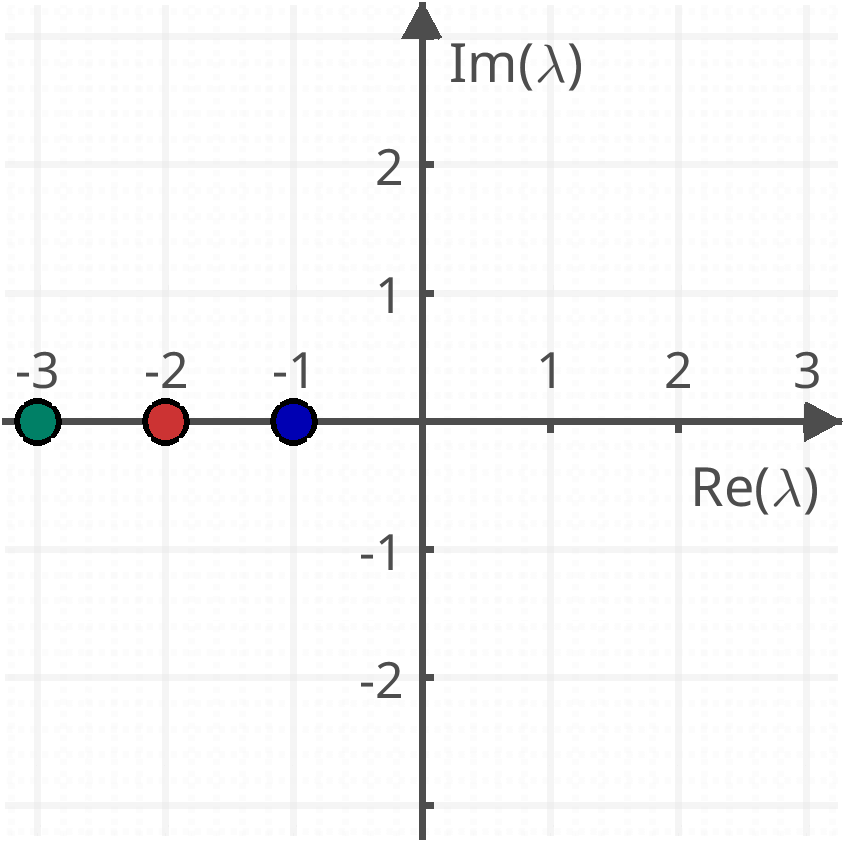
\includegraphics[width=\textwidth]{../images/task2/lambda2.png}}
		\end{minipage}
		
		\vspace{2mm} 
		
		\begin{minipage}[t]{0.68\textwidth}
			\centering
			\refstepcounter{figure}
			\small Рисунок~\thefigure: График выхода
		\end{minipage}
		\hfill
		\begin{minipage}[t]{0.29\textwidth}
			\centering
			\refstepcounter{figure}
			\small Рисунок~\thefigure: Полюса передаточной функции
		\end{minipage}
	\end{figure}
	
	Для эксперимента с полюсами
	\[
	\lambda = [-1, -2, -3]
	\]
	получены следующие характеристики переходного процесса:

	\[
	M_p = \frac{y_{\max} - y_{\infty}}{y_{\infty}} \times 100\% = \frac{1 - 1}{1} \times 100\% = 0\%
	\]
	
	
	\[
	t_p = 4.08 \text{ с}.
	\]
	
	
	\subsubsection{Эксперимент 3}
	
	
	\begin{figure}[H]
		\centering
		\begin{minipage}[c]{0.66\textwidth}
			\centering
			\raisebox{-0.5\height}{
\includegraphics[width=\textwidth]{../images/task2/y3.png}}
		\end{minipage}
		\hfill
		\begin{minipage}[c]{0.31\textwidth}
			\centering
			\raisebox{0.2\height}{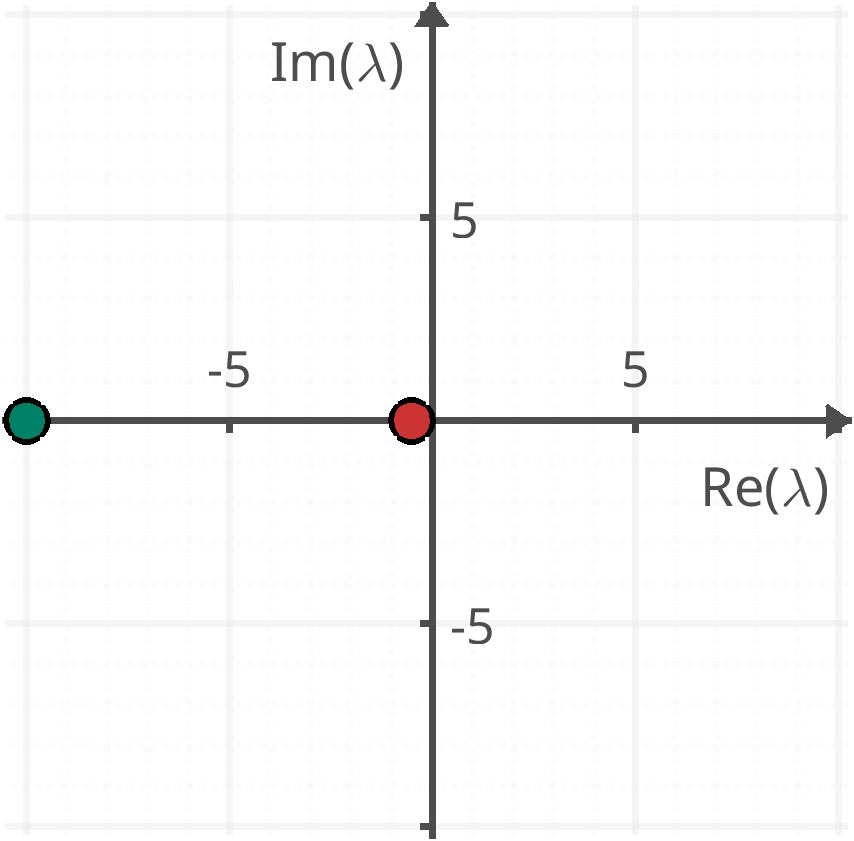
\includegraphics[width=\textwidth]{../images/task2/lambda3.png}}
		\end{minipage}
		
		\vspace{2mm} 
		
		\begin{minipage}[t]{0.68\textwidth}
			\centering
			\refstepcounter{figure}
			\small Рисунок~\thefigure: График выхода
		\end{minipage}
		\hfill
		\begin{minipage}[t]{0.29\textwidth}
			\centering
			\refstepcounter{figure}
			\small Рисунок~\thefigure: Полюса передаточной функции
		\end{minipage}
	\end{figure}
	
	
		Для эксперимента с полюсами
	\[
	\lambda = [-0.5, -0.5, -10]
	\]
	получены следующие характеристики переходного процесса:

	\[
	M_p = \frac{y_{\max} - y_{\infty}}{y_{\infty}} \times 100\% = \frac{0.99 - 0.99}{0.99} \times 100\% = 0\%
	\]
	
	
	\[
	t_p = 9.27 \text{ с}.
	\]
	
	
	
	\subsubsection{Эксперимент 4}
	
	
	\begin{figure}[H]
		\centering
		\begin{minipage}[c]{0.66\textwidth}
			\centering
			\raisebox{-0.5\height}{
\includegraphics[width=\textwidth]{../images/task2/y4.png}}
		\end{minipage}
		\hfill
		\begin{minipage}[c]{0.31\textwidth}
			\centering
			\raisebox{0.2\height}{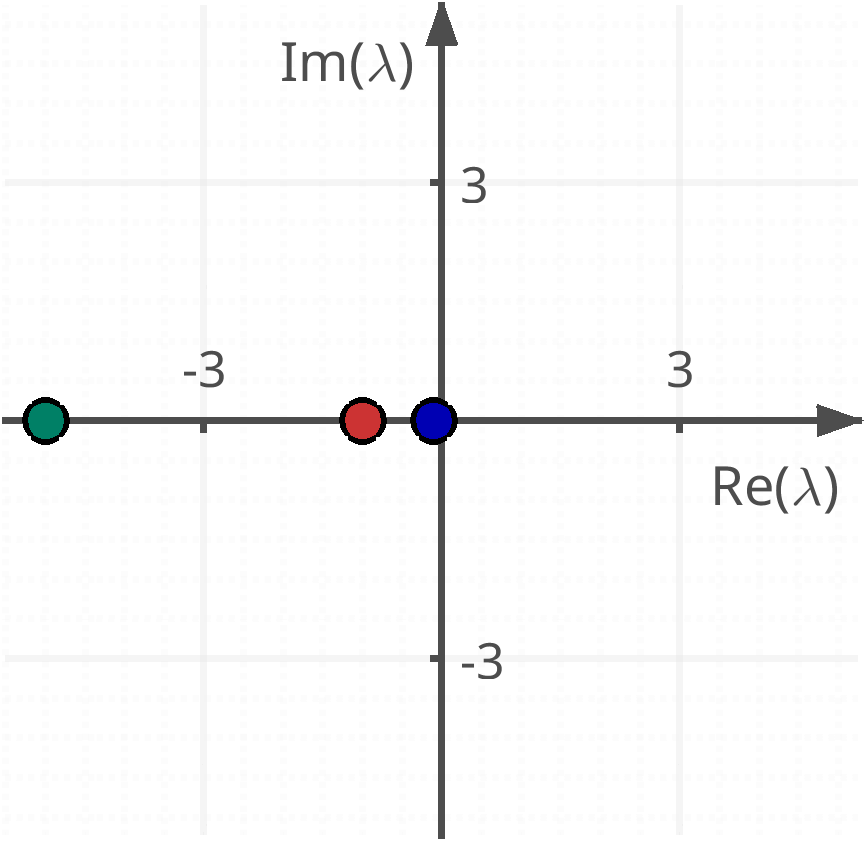
\includegraphics[width=\textwidth]{../images/task2/lambda4.png}}
		\end{minipage}
		
		\vspace{2mm} 
		
		\begin{minipage}[t]{0.68\textwidth}
			\centering
			\refstepcounter{figure}
			\small Рисунок~\thefigure: График выхода
		\end{minipage}
		\hfill
		\begin{minipage}[t]{0.29\textwidth}
			\centering
			\refstepcounter{figure}
			\small Рисунок~\thefigure: Полюса передаточной функции
		\end{minipage}
	\end{figure}
		Для эксперимента с полюсами
	\[
	\lambda = [-0.1, -1, -5]
	\]
	получены следующие характеристики переходного процесса:

	\[
	M_p = \frac{y_{\max} - y_{\infty}}{y_{\infty}} \times 100\% = \frac{0.99 - 0.99}{0.99} \times 100\% = 0\%
	\]
	
	\[
	t_p = 29.86 \text{ с}.
	\]
	
	
	\subsubsection{Эксперимент 5}
	
	
	\begin{figure}[H]
		\centering
		\begin{minipage}[c]{0.66\textwidth}
			\centering
			\raisebox{-0.5\height}{
\includegraphics[width=\textwidth]{../images/task2/y5.png}}
		\end{minipage}
		\hfill
		\begin{minipage}[c]{0.31\textwidth}
			\centering
			\raisebox{0.2\height}{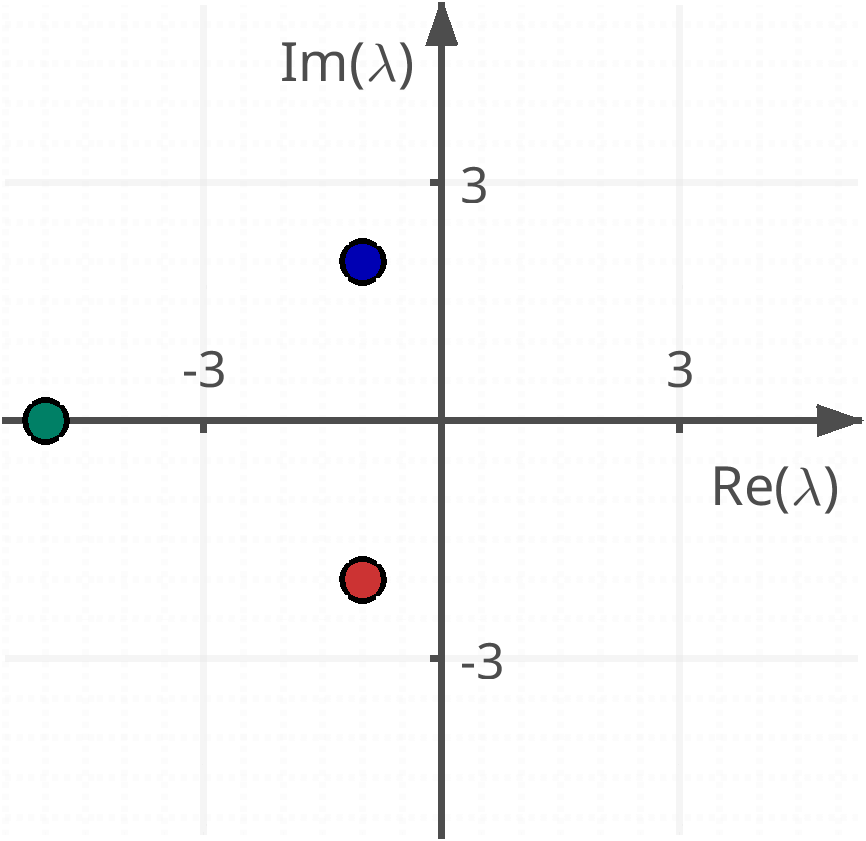
\includegraphics[width=\textwidth]{../images/task2/lambda5.png}}
		\end{minipage}
		
		\vspace{2mm} 
		
		\begin{minipage}[t]{0.68\textwidth}
			\centering
			\refstepcounter{figure}
			\small Рисунок~\thefigure: График выхода
		\end{minipage}
		\hfill
		\begin{minipage}[t]{0.29\textwidth}
			\centering
			\refstepcounter{figure}
			\small Рисунок~\thefigure: Полюса передаточной функции
		\end{minipage}
	\end{figure}
	
		Для эксперимента с полюсами
	\[
	\lambda = [-1+2i, -1-2i, -5]
	\]
	получены следующие характеристики переходного процесса:
	
	\[
	M_p = \frac{y_{\max} - y_{\infty}}{y_{\infty}} \times 100\% = \frac{1.18 - 1}{1} \times 100\% = 18\%
	\]
	
	
	\[
	t_p = 2.56 \text{ с}
	\]
	
	\[
	M_p^{\max} = e^{-\frac{\pi |\alpha|}{\beta}} \times 100\% = e^{-\frac{\pi \cdot 1}{2}} \times 100\% \approx 20.8\%.
	\]
	
	
	Полученное значение \( M_p = 18\% \) находится ниже верхней оценки, что соответствует теоретическим ожиданиям.
	
		\subsubsection{Эксперимент 6}
	
	
	\begin{figure}[H]
		\centering
		\begin{minipage}[c]{0.66\textwidth}
			\centering
			\raisebox{-0.5\height}{
\includegraphics[width=\textwidth]{../images/task2/y6.png}}
		\end{minipage}
		\hfill
		\begin{minipage}[c]{0.31\textwidth}
			\centering
			\raisebox{0.2\height}{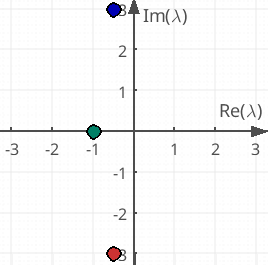
\includegraphics[width=\textwidth]{../images/task2/66.png}}
		\end{minipage}
		
		\vspace{2mm} 
		
		\begin{minipage}[t]{0.68\textwidth}
			\centering
			\refstepcounter{figure}
			\small Рисунок~\thefigure: График выхода
		\end{minipage}
		\hfill
		\begin{minipage}[t]{0.29\textwidth}
			\centering
			\refstepcounter{figure}
			\small Рисунок~\thefigure: Полюса передаточной функции
		\end{minipage}
	\end{figure}
	
		Для эксперимента с полюсами
	\[
	\lambda = [-0.5+3i, -0.5-3i, -1]
	\]
	получены следующие характеристики переходного процесса:
	
	\[
	M_p = \frac{y_{\max} - y_{\infty}}{y_{\infty}} \times 100\% = \frac{1.03 - 1}{1} \times 100\% = 3\%
	\]
	
	
	\[
	t_p = 3.13 \text{ с}
	\]
	
	\[
	M_p^{\max} = e^{-\frac{\pi |\alpha|}{\beta}} \times 100\% = e^{-\frac{\pi \cdot 0.5}{3}} \times 100\% \approx 59.2\%.
	\]
	
	
	Полученное значение \( M_p = 3\% \) находится ниже верхней оценки, что соответствует теоретическим ожиданиям.
	
	
	\subsubsection{Эксперимент 7}
	
	
	\begin{figure}[H]
		\centering
		\begin{minipage}[c]{0.66\textwidth}
			\centering
			\raisebox{-0.5\height}{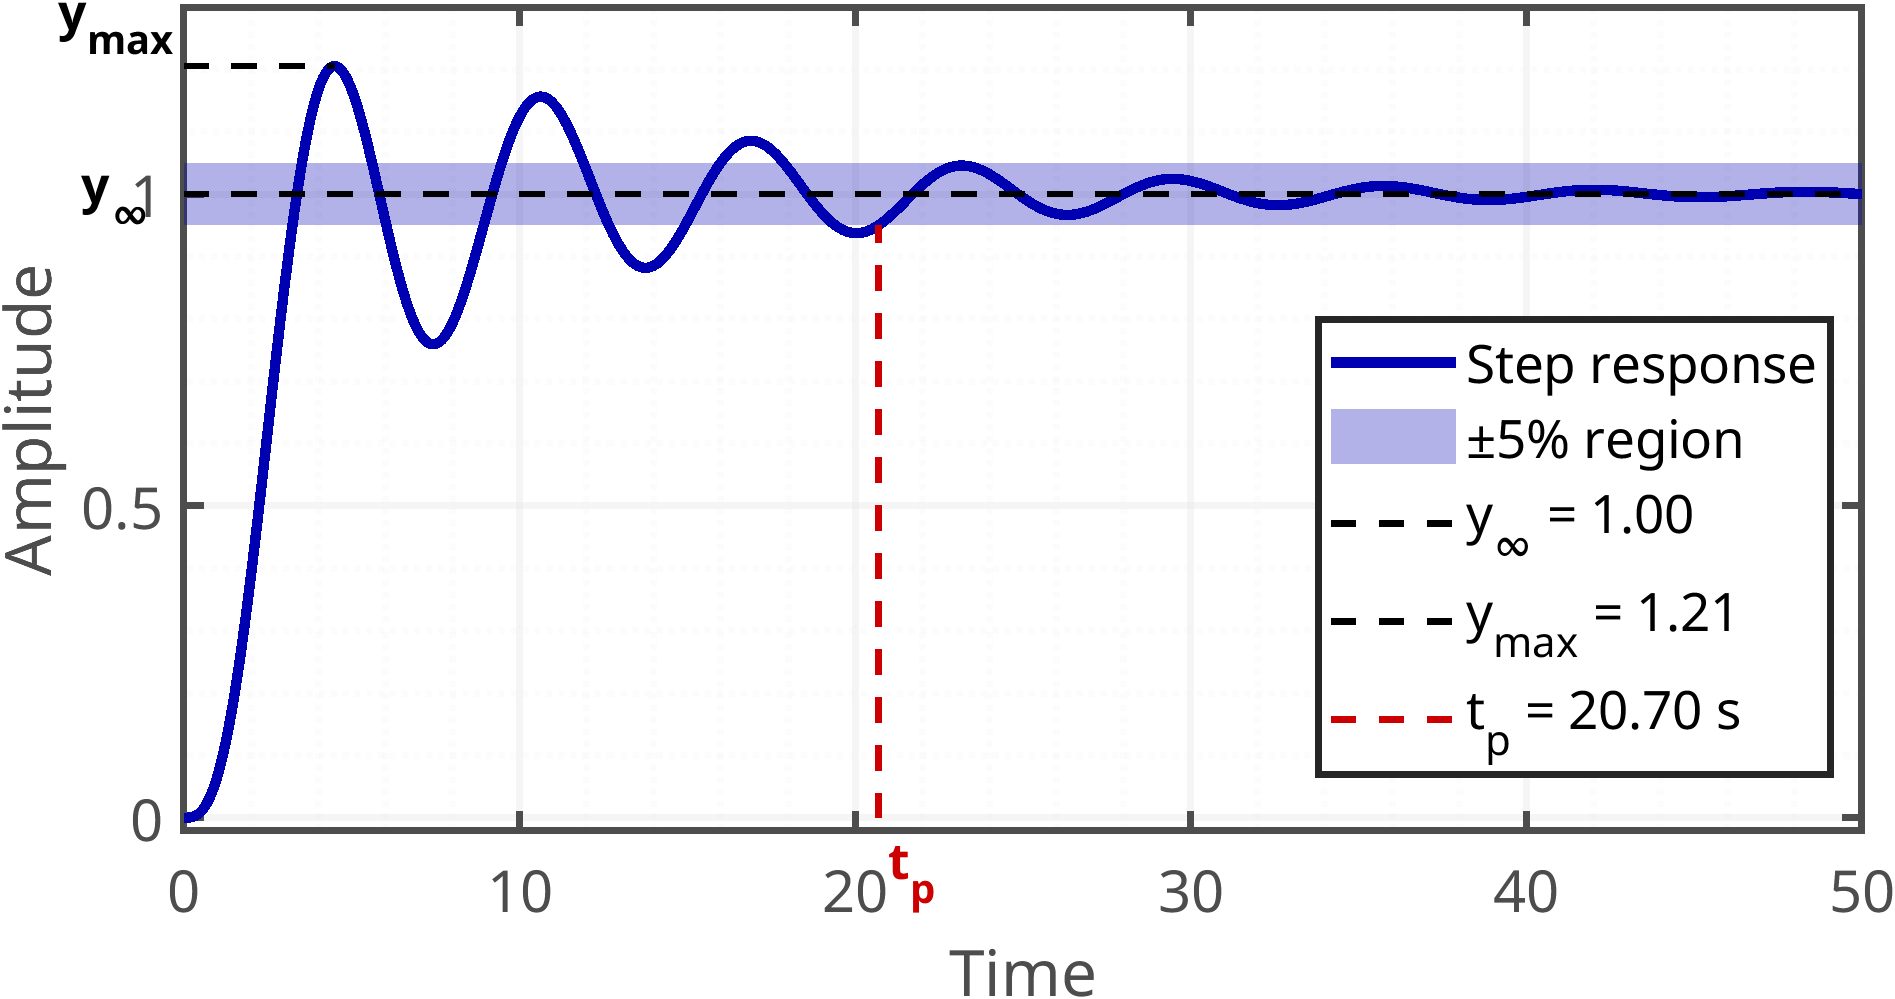
\includegraphics[width=\textwidth]{../images/task2/y7.png}}
		\end{minipage}
		\hfill
		\begin{minipage}[c]{0.31\textwidth}
			\centering
			\raisebox{0.2\height}{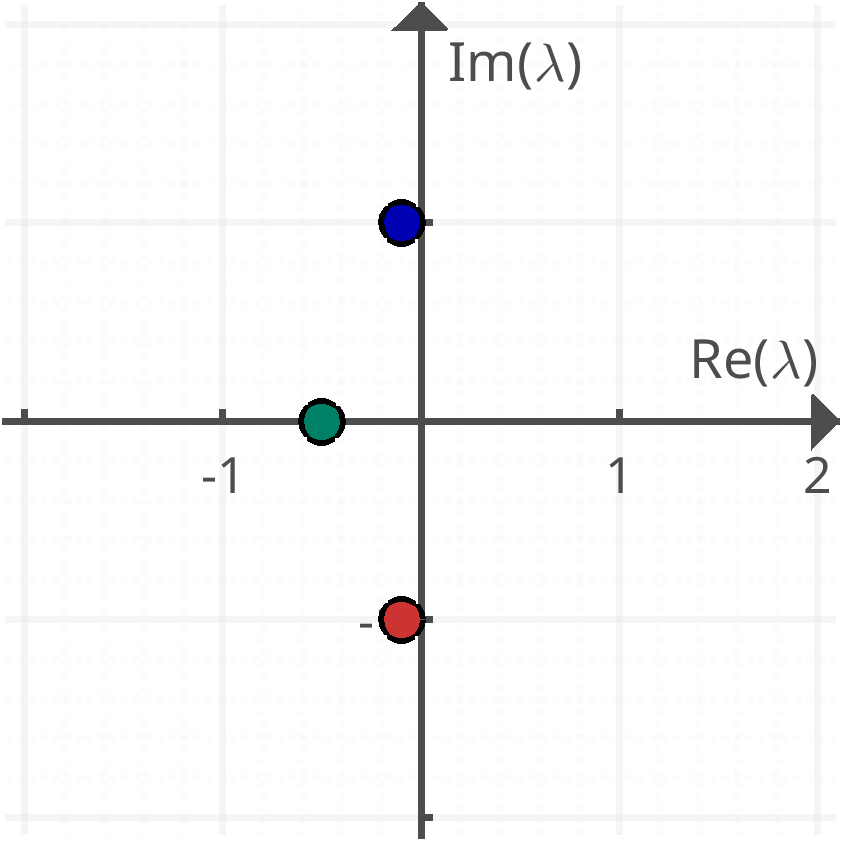
\includegraphics[width=\textwidth]{../images/task2/lambda7.png}}
		\end{minipage}
		
		\vspace{2mm} 
		
		\begin{minipage}[t]{0.68\textwidth}
			\centering
			\refstepcounter{figure}
			\small Рисунок~\thefigure: График выхода
		\end{minipage}
		\hfill
		\begin{minipage}[t]{0.29\textwidth}
			\centering
			\refstepcounter{figure}
			\small Рисунок~\thefigure: Полюса передаточной функции
		\end{minipage}
	\end{figure}
	
		Для эксперимента с полюсами
	\[
	\lambda = [-0.1+1i, -0.1-1i, -0.5]
	\]
	получены следующие характеристики переходного процесса:
	
	\[
	M_p = \frac{y_{\max} - y_{\infty}}{y_{\infty}} \times 100\% = \frac{1.21 - 1}{1} \times 100\% = 21\%
	\]
	
	
	\[
	t_p = 20.7 \text{ с}
	\]
	
	\[
	M_p^{\max} = e^{-\frac{\pi |\alpha|}{\beta}} \times 100\% = e^{-\frac{\pi \cdot 0.1}{1}} \times 100\% \approx 73\%.
	\]
	
	
	Полученное значение \( M_p = 21\% \) находится ниже верхней оценки, что соответствует теоретическим ожиданиям.
	
	\subsubsection{Эксперимент 8}
	
	
	\begin{figure}[H]
		\centering
		\begin{minipage}[c]{0.66\textwidth}
			\centering
			\raisebox{-0.5\height}{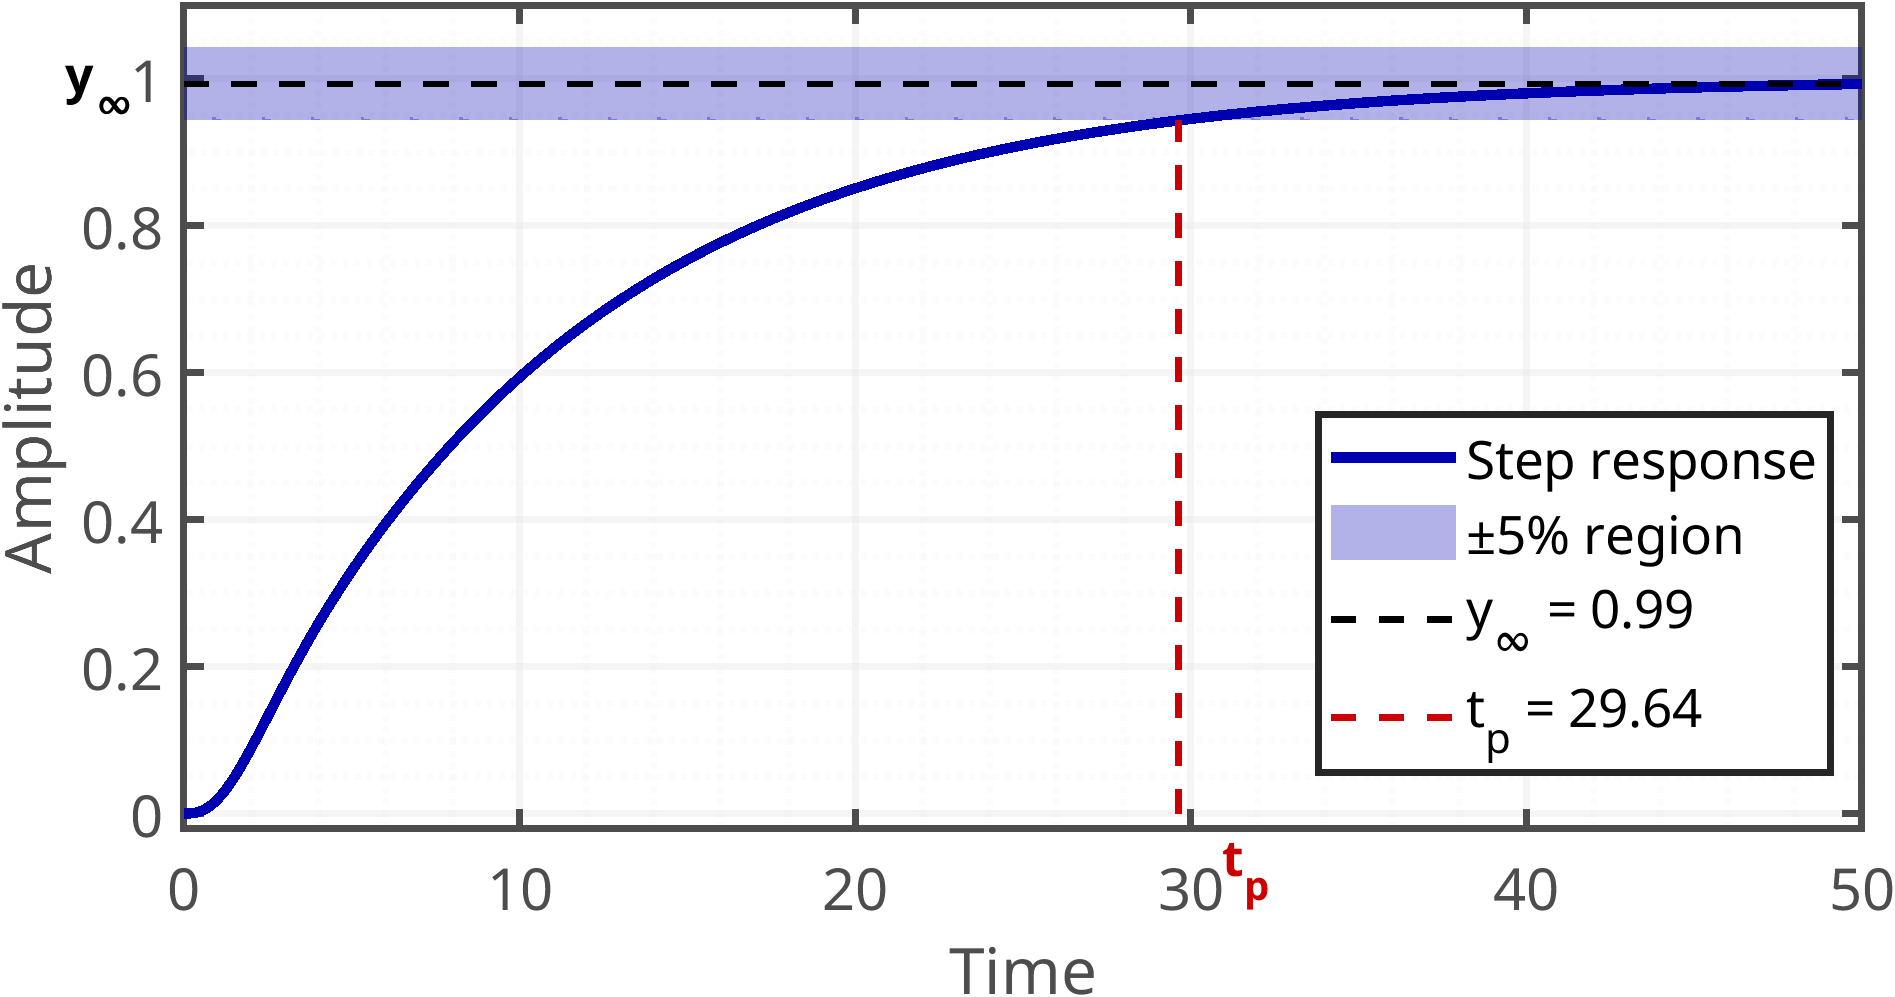
\includegraphics[width=\textwidth]{../images/task2/y8.png}}
		\end{minipage}
		\hfill
		\begin{minipage}[c]{0.31\textwidth}
			\centering
			\raisebox{0.2\height}{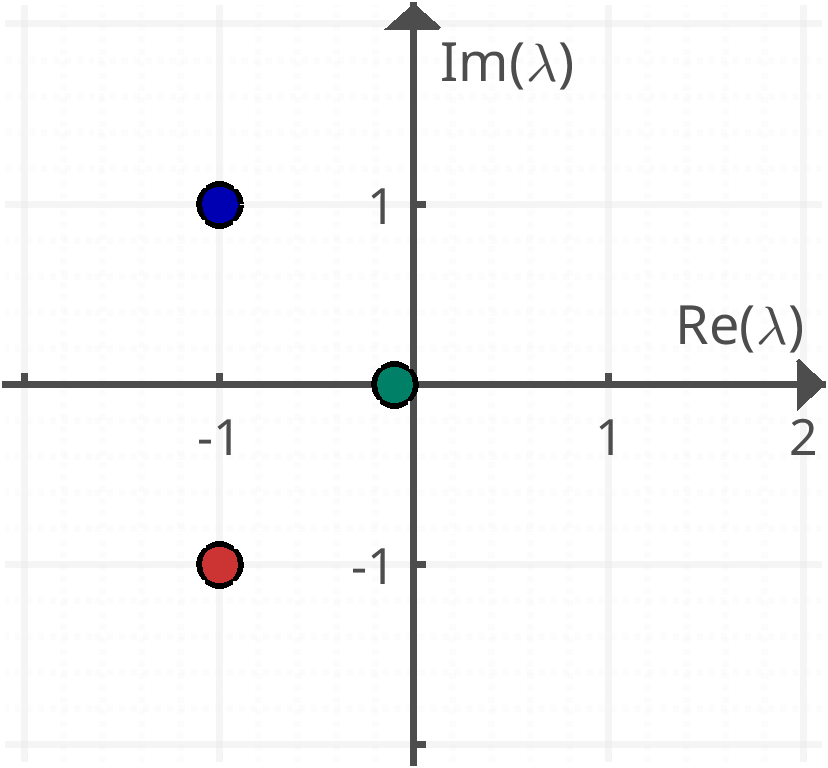
\includegraphics[width=\textwidth]{../images/task2/lambda8.png}}
		\end{minipage}
		
		\vspace{2mm} 
		
		\begin{minipage}[t]{0.68\textwidth}
			\centering
			\refstepcounter{figure}
			\small Рисунок~\thefigure: График выхода
		\end{minipage}
		\hfill
		\begin{minipage}[t]{0.29\textwidth}
			\centering
			\refstepcounter{figure}
			\small Рисунок~\thefigure: Полюса передаточной функции
		\end{minipage}
	\end{figure}
	
		Для эксперимента с полюсами
	\[
	\lambda = [-1+1i, -1-1i, -0.05]
	\]
	получены следующие характеристики переходного процесса:
	
	\[
	M_p = \frac{y_{\max} - y_{\infty}}{y_{\infty}} \times 100\% = \frac{0.99 - 0.99}{0.99} \times 100\% = 0.00\%
	\]
	
	
	\[
	t_p = 29.64 \text{ с}
	\]
	
	\[
	M_p^{\max} = e^{-\frac{\pi |\alpha|}{\beta}} \times 100\% = e^{-\frac{\pi \cdot 1}{1}} \times 100\% \approx 4.3\%.
	\]
	
	
	Полученное значение \( M_p = 0\% \) находится ниже верхней оценки, что соответствует теоретическим ожиданиям.
	
	
	\newpage
	
	\textbf{Итог: }	
	На основе рассмотренных наборов полюсов \(\lambda_1, \lambda_2, \lambda_3\) видно следующее:
	
	\begin{itemize}
		\item Если все полюса вещественные и отрицательные (например, эксперименты 1–4), система ведёт себя устойчиво с плавным затуханием. Чем больше по модулю значения полюсов, тем быстрее затухание.
		\item При кратных полюсах (эксперимент 1) процесс затухания равномерный и без колебаний.
		\item Если есть комплексно-сопряжённые полюса (эксперименты 5–8), система начинает колебаться. Частота колебаний связана с мнимой частью \(\beta\), а скорость затухания -- с действительной частью \(\alpha\).
		\item Чем ближе действительная часть к нулю (например, эксперимент 7), тем медленнее затухают колебания.
	\end{itemize}

	
	\newpage
	\section{Вывод}
	
	В лабораторной работе я исследовала вынужденное движение, а также показатели качества системы. Установила, что  устойчивость системы зависит от ее параметров, а качество переходного процесса -- от расположения полюсов передаточной функции на комплексной плоскости.


	Материалы работы: \href{https://github.com/decadeos/ITMO/tree/master/3_course/lsau/lab3}{\texttt{github.com}}
	
\end{document}